% This is "sig-alternate.tex" V2.0 May 2012
% This file should be compiled with V2.5 of "sig-alternate.cls" May 2012
% For tracking purposes - this is V2.0 - May 2012

\documentclass[final]{sig-alternate}

\usepackage[english]{babel}
\usepackage{amsmath}
\usepackage{graphicx}
\usepackage[colorinlistoftodos,obeyFinal]{todonotes}
\usepackage[ruled]{algorithm}
\usepackage[table]{colortbl}
\usepackage{algpseudocode}
\usepackage{acronym}
\usepackage{url}
\usepackage{textcomp}

\acrodef{POD}{Programmable Output Device}
\acrodef{PC}{Personal Computer}
\acrodef{DAQ}{Data Acquisition}
\acrodef{DAQ}{Data Acquisition}
\acrodef{MBCT}[MBCT]{Model-Based Clinical Trial}
\acrodef{RCT}{Randomized Controlled Trial}
\acrodef{CT}{Clinical Trial}
\acrodef{VT}{Ventricular Tachycardia}
\acrodef{VF}{Ventricular Fibrillation}
\acrodef{SVT}{SupraVentricular Tachycardia}
\acrodef{PRLW}[PRL+W]{PR Logic + Wavelet}
\acrodef{EGM}{electrogram}
\acrodef{ECG}[ECG]{electrocardiogram}
\acrodef{ICD}[ICD]{Implantable Cardioverter Defibrillator}
\acrodef{AGC}[AGC]{automatic gain control}
\acrodef{AAS}[AAS]{auto-adjusting sensitivity}
\acrodef{NSR}[NSR]{normal sinus rhythm}

\newboolean{DRAFT}
\setboolean{DRAFT}{FALSE}
\newboolean{TENPAGES}
\setboolean{TENPAGES}{FALSE}

\usepackage{tikz}
\newcommand*\circled[1]{\tikz[baseline=(char.base)]{
		\node[shape=circle,draw,inner sep=2pt] (char) {#1};}}
\newcommand{\smallcaption}[1]{\caption{\small #1}}
\newcommand{\headline}[1]{\ifthenelse{\boolean{DRAFT}}{\textcolor{blue}{#1}}{#1}}
\newcommand\Mark[1]{\textsuperscript#1}
\newcommand{\mynote}[2]{\todo[inline]{#1: #2}}

\graphicspath{{figures/}}
\linespread{0.97}
\begin{document}
%
% --- Author Metadata here ---
\conferenceinfo{ICCPS}{2016 Vienna, Austria}
%\CopyrightYear{2007} % Allows default copyright year (20XX) to be over-ridden - IF NEED BE.
%\crdata{0-12345-67-8/90/01}  % Allows default copyright data (0-89791-88-6/97/05) to be over-ridden - IF NEED BE.
% --- End of Author Metadata ---

\title{Model-Based Clinical Trials for Medical Devices}

\numberofauthors{5} 
%

\author{
	Houssam Abbas\Mark{1}, Zhihao Jiang\Mark{1}, Kuk Jin Jang\Mark{1}, Marco Beccani\Mark{1}\\
	\and
	Jackson Liang\Mark{2}, Sanjay Dixit\Mark{3}, and Rahul Mangharam\Mark{1}\\
	\begin{tabular}[t]{@{}c@{}}
		\\
		\affaddr{\normalsize \Mark{1}Dept. of Electrical and Systems Eng.}\\
		\affaddr{\normalsize University of Pennsylvania}\\
		\email{\normalsize\{habbas, zhihaoj, jangkj, beccani, rahulm\}@seas.upenn.edu}\\
	\end{tabular}\nobreak\qquad
	\begin{tabular}[t]{@{}c@{}}
		\\
		\affaddr{\normalsize \Mark{2}Cardiovascular Division,~\Mark{3}Cardiac Electrophysiology}\\
		\affaddr{\normalsize Hospital of the University of Pennsylvania}\\
		\email{\normalsize \{jackson.liang, sanjay.dixit\}@uphs.upenn.edu}
	\end{tabular}
}


\maketitle

%%% A category with the (minimum) three required fields
%%\category{H.5.1}{Computing methodologies}{Modeling and simulation}[Model development and analysis]
%%%A category including the fourth, optional field follows...
%%\category{L.2}{Applied computing}{Life and medical sciences}
%%
%%\terms{Medical devices, life-critical CPS, model-based clinical trials, heart modeling, arrhythmias, ICDs}
\begin{abstract}
Ventricular Fibrillation is a disorganized electrical excitation of the heart that results in inadequate blood flow to the body.
It usually ends in death within seconds.
The most common way to treat the symptoms of fibrillation is to implant a medical device, known as an \emph{Implantable Cardioverter Defibrillator} (ICD), in the patient's body.
Model-based verification can supply rigorous proofs of safety and efficacy. 
In this paper, we build a hybrid system model of the human heart+ICD closed loop, and show it to be a \yhl{STORMED system, a class of o-minimal hybrid systems that admit finite bisimulations.}
In general, it may not be possible to compute the bisimulation.
We show that approximate reachability can yield a finite \emph{simulation} for STORMED systems, which improves on the existing verification procedure.
In the process, we show that certain compositions respect the STORMED property.
Thus it is possible to model check important formal properties of ICDs in a closed loop with the heart, such as delayed therapy, missed therapy, or inappropriately administered therapy. 
The results of this paper are theoretical \yhl{and motivate the creation of concrete model checking procedures for STORMED systems.}
\end{abstract}

%Ventricular Fibrillation is a disorganized electrical excitation of the heart that results in inadequate blood flow to the body.
%It usually ends in death within a few seconds.
%The most common way to treat the symptoms of fibrillation is to implant a medical device, known as an Implantable Cardioverter Defibrillator (ICD), in the patient's body.
%Model-based verification can play a crucial role in ICD development.
%In this paper, we build a hybrid system model of the human heart+ICD closed-loop system, and show that it admits a finite bisimulation by showing it to be a STORMED hybrid system.
%In general, it may not be possible to compute the bisimulation.
%We show that approximate reachability can yield a finite \emph{simulation} for STORMED systems, which improves on the existing verification procedure.
%In the process, we show that certain compositions respect the STORMED property.
%Thus it is possible to model check important formal properties of ICDs in a closed loop with the heart, such as delayed therapy, missed therapy, or inappropriately administered therapy. 
%The results of this paper are theoretical, since no model checkers exist for STORMED systems. 
%In future work we will implement a procedure for model checking the heart+ICD loop.
\section{Introduction}
\label{introduction}

%\todo[inline]{stress the timing aspect more}
Implantable medical devices such as pacemakers are designed to improve physiological conditions with very little human intervention. 
Their ability to autonomously affect the physiological state of the patient makes the medical devices safety-critical, and sufficient evidence for their safety and efficacy should be provided before the devices can be implanted in the patients. Medical devices increasingly rely on software, and device function and their clinical performance can be affected by seemingly minor changes to software.
%As more functionality is added to the devices
\footnote{In what follows, the word `device' is used to refer to the software of the device.}
%, the complexity of the software component of the device is increasing dramatically, leading to a large number of potential safety violations because of software bugs. 

Over the course of the past four decades, cardiac rhythm management devices such as pacemakers and implantable cardioverter defibrillators (ICD) have grown in complexity and now have more than 80,000 to 100,000 lines of software code~\cite{pauljones}. In 1996, 10\% of \emph{all} medical device recalls were caused by software-related issues and this rose to 15\% between 2003-2012~\cite{recall_stats,killedbycode}. There is currently no standard for testing, validating, and verifying the software for implantable medical devices~\cite{fda1,fda3}.

There are two categories of device bugs: 
1) the device may fail to conform to its \emph{specifications}, that is, the prescription of how it should react to certain inputs.  
2) the device may fail to improve the conditions of the patient as promised, even if it conforms to its specifications. 
The desired physiological conditions that the closed-loop system should achieve are captured in the \emph{physiological requirements}; for example, for a pacemaker, the heart rate should always be maintained above a certain threshold. 
%In what follows, the word `requirement' always refers to such physiological requirements.
%Note that requirements are about \emph{the closed-loop system}: they prescribe the behavior of both device and environment (e.g. both pacemaker and heart).

Bugs in the first category (non-conformance to specification) can be detected via systematic and extensive open-loop testing in which a set of input sequences is fed to the device, and its output is compared with the expected output.
Bugs in the second category (violation of physiological requirements), on the other hand, require the availability of the \emph{closed-loop system}, which consists of the device and its environment.
For instance, the pacemaker and the heart as its environment. 
In the medical device industry, closed-loop verification of the physiological requirements is mostly performed in terms of clinical trials, in which the actual devices are implanted in human subjects over an extended duration.
Unfortunately, because of the extremely high cost of clinical trials (several million dollars and spanning several years~\cite{trial_cost}), the amount and variety of human subjects during the clinical trials are limited, which reduces the opportunity to find bugs. 
Moreover, clinical trials are often conducted at the final design stage. Fixing bugs at this stage is very costly.

Closed-loop model checking enables closed-loop evaluation of the physiological requirements at an earlier design stage, which requires formal model(s) of the physiological environment. 
%Depending on the formalism used to model the environment (and device) and the language used to express the requirements, this allows the usage of formal methods to perform the verification.
%Formal environment modeling introduces new challenges that do not arise when modeling the device alone, and this paper aims at addressing these issues in the context of pacemaker verification.
%In the rest of this paper, we speak therefore of pacemaker as the Device Under Verification (DUV) and of the heart as being the environment, but it is understood that the discussion carries more broadly, with possible domain-specific adjustments.
In closed-loop model checking, there is only one device model. 
However there can be a large number of environmental conditions which require different models to represent them. For instance, a heart with atrial flutter has an additional conduction pathway that is not present in a healthy heart, causing fast atrial rate. The timing and structural differences of different heart conditions should be distinguished in corresponding heart models.
%\todo[inline]{should we give an example of a heart condition?}
A set of initial models of the environment can be constructed but the set is inherently incomplete because of the large number of environment conditions and their combinations. 
As a result, performing model checking using every model in the set cannot ensure full coverage of the environmental conditions. 

In this paper, domain-specific over-approximation rules are developed that produce abstract models that not only cover explicitly modeled environment conditions, but also cover timing behaviors and conditions not modeled in the set of initial models. 
The abstract models can be then used for closed-loop model checking of the device model. 
If the closed-loop system satisfies a requirement, the device under verification satisfies the requirement under environment conditions covered by the abstract models. 
However, if the requirement is not satisfied, the model checker returns a counter-example. 
In device modeling, the counter-example is considered \emph{spurious} if it can not be produced by the device (as shown in (\figref{distinction}(a)).
However in environment modeling, even if the counter-example can not be produced by any of the initial environment models, it might still be a physiologically valid behavior.
Thus the validity of a counter-example cannot be determined by refining the environment model, but can ultimately only be determined by domain experts. 

Counter-examples returned from abstract models can be difficult to interpret by domain experts.
One abstract counter-example could be produced by multiple physiologically valid conditions, which causes ambiguity.
Thus, a rigorous framework is necessary to balance the need to cover a wide range of environmental conditions and the need to provide counter-examples to the physicians within their physiological context.

Another challenge for closed-loop model checking of medical devices is the amount of domain expertise needed during: 1) physiological modeling, 2) model abstraction and refinement, and 3) checking the validity of counter-examples.
Thus the framework must also allow non-domain experts to perform verification (item 2 above),
and establish `hand-off' points where the results of verification can be handed back 
to the experts for interpretation.

\begin{figure}[!t]
		\centering
		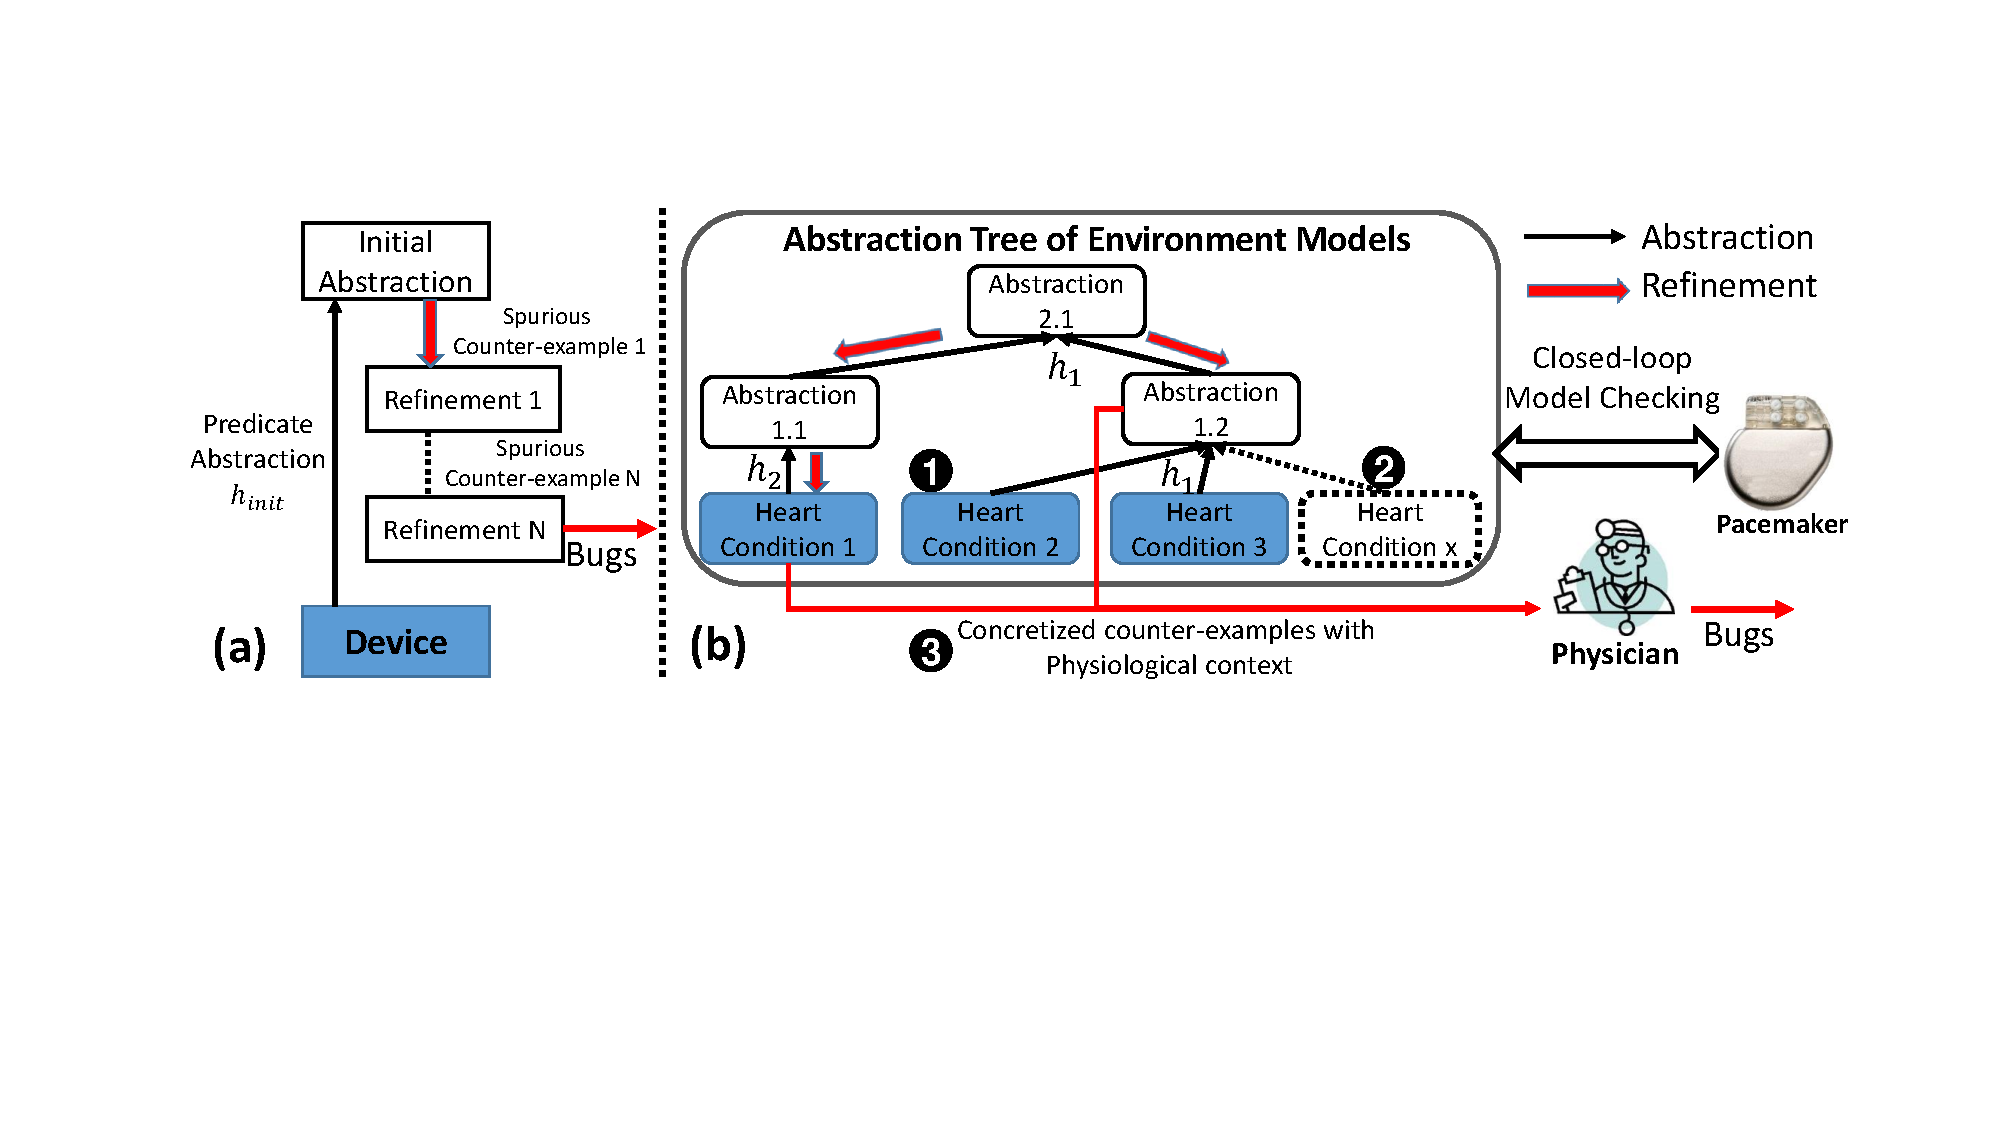
\includegraphics[width=\textwidth]{figs/distinction.pdf}
		%\vspace{-5pt}
		\caption{\small (a) Device modeling with CEGAR framework (b) Closed-loop model checking with environment abstraction tree.}% The initial set of heart conditions are first abstracted and/or merged using abstraction rules $h_1,h_2$ (Marker 1). The abstract model is first used for closed-loop model checking. When a property violation happens, refined models in the abstraction tree are used for model checking. The most concrete counter-examples may be available in the initial model(s) (Marker 2). In the scenario where counter-examples do not exist in explicitly modeled Heart condition 2 and 3, the counter-example in Abstraction 1.2 may correspond to a valid heart condition introduced during abstraction $h_1$. The physician decides the validity of the counter-examples.}
		  \vspace{-10pt}
		\label{fig:distinction}
\end{figure}


\subsection{Contributions}
In this paper a framework is proposed for environment modeling in closed-loop model checking of medical device software.
The cardiac pacemaker is used as an example of applying this framework.
An expandable set of timed-automata heart models are first developed to represent different physiological conditions (\figref{distinction} Marker 1).
A set of domain-specific abstraction rules are then developed based on physiological knowledge, which help ensure the physiological relevance of the behaviors introduced into the abstract models (\figref{distinction} Marker 2).
Then the rules are applied to the initial set of physiological models to obtain an abstraction tree, which will be used for closed-loop model checking of the pacemaker. 
A straightforward search procedure is then used to conduct model checking using suitable heart models and return the most concrete and unambiguous counter-examples to the physicians for analysis (\figref{distinction} Marker 3).
In this framework, physiological knowledge is only needed when constructing the initial model set and when analyzing counter-examples. 
The application of the physiological abstraction rules and the verification procedure can be automated.
The proposed method can potentially be generalized to other domains in which the device operates in a large variety of environmental conditions.
\subsection{Related Work}
%\todo[inline]{complete}
Counter-Example Guided Abstraction Refinement (CEGAR) \cite{CEGAR} has been proposed to over-approximate the behaviors of the device using predicate abstraction (\figref{distinction}.(a)).
%Upon property violation the abstract counter-example is checked for its validity on the actual system. If the counter-example is \emph{spurious} the model is then refined to eliminate the spurious counter-example. 
%This process is then continued on the refined model until either a valid counter-example returns or no counter-examples are returned. 
CEGAR works well during device modeling, however, it cannot be applied to environment modeling for two reasons: 1)~predicate abstraction does not guarantee the validity of behaviors introduced into the model. In fact, for device modeling, all additional behaviors introduced into the abstract model are spurious. 2)~the validity of a counter-example cannot be checked automatically as in device modeling. 

Proof-based approaches have also been applied to verify  abstractions and refinements of pacemaker specification using Event-B~\cite{eventb}. However, the authors did not take into account environment behaviors thus the framework cannot be used for verifying physiological requirements.  

Physiological modeling of cardiac activities has been studied at various levels for different applications. In \cite{natalia}, the electrical activity of the heart is modeled with high spatial fidelity to study the mechanisms of cardiac arrhythmia. In \cite{radu}, formal abstractions of cardiac tissue have been studied to reduce the complexity of the heart tissue model. However, these two models do not focus on the interaction with the pacemaker, therefore cannot be used for closed-loop model checking. In \cite{marta}, hybrid automata models of the heart has been used to capture the complex beat-to-beat dynamics of the heart tissue. However the model cannot be used to cover behaviors across different heart conditions.

In previous work \cite{sttt13} a set of formal heart models covering various heart conditions at different abstraction levels was developed, and closed-loop model checking was performed on models of implantable pacemakers. 
However, the physiological knowledge required during each step of closed-loop model checking prevents the method to be practical.


%During the closed-loop model checking, the most abstract model(s) that are appropriate to the requirement are automatically selected as the initial environment models. If the requirement is satisfied, the system is safe under the environment conditions covered by the initial environment models. If the requirement is violated in certain initial environment model, the children of the model in the abstraction tree are used for model checking until 1) the leaves of the tree is reached, or 2) there is no violations in the child nodes. The counter-examples obtained at the most refined models are returned to the physician for validity check. This process is automated so that no domain knowledge is required for the person who performs model checking. It also ensures the most concrete counter-examples with unambiguous physiological context are returned to the physician for analysis. 
%The first challenge in closed-loop model checking of pacemakers is that the human heart displays a large number of different conditions, henceforth referred to as `physiological conditions'.
%E.g., one heart may display \emph{atrial fibrillation} where the upper chambers of the heart (the atria) produce an exceedingly fast beat that prevents proper blood pumping.
%Another heart may display Premature Ventricular Contraction (PVC) where a location in the ventricles produces electrical impulses at erratic time instants.\Hao{I don't think these two conditions make sense to the reader}
%Each such condition will require its own formal model, and some models may display more than one condition.
%In this paper, we build such a set of formal heart models using the timed automata formalism in Section ???.
%Performing model checking with each model separately, we seek a method that can combine models, and perform model checking on the merged model. 
%The combination of models must be such that if the merged model is correct (according to the requirements) then so is every model that was combined into it.
%We present \emph{abstraction rules} in Section ?? which allow us to do precisely that.

%This initial set of models will necessarily be \emph{incomplete} because the number of physiological conditions is too large, and some of the conditions are too ill-understood for modeling.
%Thus, unlike system modeling in which one typically starts from one ground truth model to be verified, our starting point is an \emph{incomplete set of environment models}.
%Because of this incompleteness, we seek abstraction rules that introduce new \emph{physiologically meaningful} behavior which might actually be produced by heart models not in the initial set.
%These then correspond to heart conditions not taken explicitly into account. 
%This provides a second motivation for the domain-specific abstraction rules $R$ in Section ???, which can be thought of as relaxations of the conditions governing the model's behavior. 
%Like predicate abstraction, they produce models that over-approximate the behavior of the model they are applied to (i.e., $\beh(R(M)) \supset \beh(M)$).
%However, the new behavior they introduce might not be spurious. 
%We demonstrate such a case in Section ???.
%If model checking returns a counter-example on $R(M)$, the physician can decide whether this is actually physiologically plausible behavior and therefore the pacemaker needs to be debugged, or this is indeed spurious and should be thrown out (and the abstraction refined).
%
%Note this is different from classical predicate abstraction [???], which adds behavior in a domain-agnostic fashion. In fact, predicate abstraction is a fist step in the timed automata model checking procedure as presented in [ALur and Dill 1994].
%Our abstraction rules are used to combine and and abstract models \emph{prior} to model checking.
%%tttt
%
%\subsubsection{Contributions}
%In this paper we propose a framework for environment modeling and model checking of medical device software, in particular, pacemakers.
%Specifically, we present several extended timed automata models of various heart conditions in Section ???. 
%We define domain-specific abstraction rules for these models, and demonstrate how these can be applied to gradually add physiologically meaningful behavior in Section ???. 
%Using the models and the rules, we build an abstraction tree which serves to perform model checking of physiological requirements for the heart+pacemaker closed loop in Section ???.
%We illustrate the approach via case studies in Section ???, and conclude in Section ???
%

%

\section{Clinical trials and RIGHT}
\label{sec:rcts}

At the clinical trial stage (Fig.~\ref{fig:spectrum}), the objective is no longer to find bugs in the device: it is, rather, to evaluate the safety and efficacy of the validated device on humans. 
\acp{RCT} are the gold standard for evaluating the safety and efficacy of a new medical device \cite{FriedmanFD10_ClinicalTrials}.
They constitute the only time prior to market use where the effects of the device on humans are actually observed, and are legally mandated for new high-risk medical devices like \acp{ICD}.
%It is important to understand how a typical RCT proceeds to appreciate where CPS modeling can help in that process.
%Very broadly, in an \ac{RCT}, a new treatment also known as the \emph{intervention}, is compared to the current standard of care, commonly known as the \emph{control}.
%For example, two competing ICDs are compared.
%Each patient recruited to the trial is randomly assigned to either the intervention or the control group and undergoes the corresponding treatment.
%At the end of the trial, any clinically relevant differences between the two groups are evaluated to determine if they are statistically significant.
The planning and execution of an \ac{RCT} requires carefully navigating a number of technical, logistical and ethical issues to obtain reliable and statistically significant results.

Because of the very high cost of \acp{RCT} in terms of money, time, and the risk of harm they present to enrolled patients, our focus in this paper is on the use of CPS models, formalized in an \ac{MBCT}, \emph{to validate the assumptions made by the investigators and thus increase the chances of success of an \ac{RCT}}.
We illustrate our approach by applying it to the Rhythm ID Going Head-to-Head Trial (RIGHT) \cite{GoldABBTB11_RIGHTresults}, which we present next.
\subsection{The RIGHT trial}
\label{sec:right}
We first provide a brief background to better understand RIGHT (see Fig.\ref{fig:icd}). Tachycardias (abnormally elevated heart rates) can be divided into \acp{VT}, which originate in the heart's ventricles, 
and \acp{SVT}, which originate above the ventricles.
A sustained \ac{VT} can be fatal, while an \ac{SVT} is typically non-fatal.
The therapy applied by the ICD often takes the form of a high-energy electric shock.
The shock can be pro-arrhythmic
\mynote{SD}{replaced pro-arrhythmic with 'quite uncomfortable'. We got pro-arrhythmic effect from Pinksy et al. "The Proarrhythmic Potential of Implantable Cardioverter-Defibrillators", 1995. Is it out-dated? It was cited in RIGHT 2006. }, and was even linked to increased morbidity \cite{shock_mortality}.
Therefore, one of the biggest challenges for ICDs is to guarantee shock delivery for \acp{VT}, and simultaneously reduce inappropriate shocks during \acp{SVT} \cite{Ellenbogen11_Pacingbook}.

RIGHT is a trial that sought to compare the VT/SVT discrimination abilities of two algorithms \cite{GoldABBTB11_RIGHTresults}: 
the Rhythm ID detection algorithm found in Boston Scientific's Vitality II ICDs~\cite{compass},
and the PR Logic + Wavelet (PRL+W) detection algorithm found in a number of Medtronic's ICDs (Medtronic Maximo,
Marquis, Intrinsic, Virtuoso, or Entrust ICD).
%\mynote{SD}{make sure to list all the Boston Scientific and Medtronics ICD models that use each of these algorithims. This is very important}
%The investigators chose the following primary question: is there a difference in time-to-first inappropriate therapy between the two ICDs?
\emph{Inappropriate therapy} was defined as therapy applied to an arrhythmia other than \ac{VT} or \ac{VF} (\ac{VF} is a type of \ac{VT}).
RIGHT enrolled 1962 patients and ran for approximately five years.
It was fully sponsored by Boston Scientific. 

One of the trial's assumptions was that Rhythm ID would reduce the risk of inappropriate therapy by 25\% over PRL+W~\cite{Berger06_RIGHT}.
The outcome of the trial~\cite{GoldABBTB11_RIGHTresults}, however, was that patients implanted with ICDs running Rhythm ID had a \emph{\textbf{34\% risk increase}} of inappropriate therapy as compared to patients implanted with \acp{ICD} running PRL+W. 
This result  is the opposite of the effect hypothesized by the trial investigators. 
In this paper, we design an \ac{MBCT} to test early and quickly whether the hypothesized effect holds by comparing the two ICDs on a large \emph{synthetic} cohort.\\\\
\textbf{\emph{Organization:}} In the following sections we describe the building blocks of the MBCT: modeling the heart, processing 100's of real patients' data, mapping the timing and morphology components of the signal to a heart model we developed, generating a population of 10,000+ synthetic heart models, implementing the device algorithms and conducting multiple trials for the comparative rate of inappropriate therapy, condition-level rates and evaluating the effect of device parameters on discrimination rates.

%Note that these differences in inappropriate therapy were confined to single-chamber ICDs.

%The patients were randomized to two groups: the intervention group were implanted with Vitality II ICDs which ran the Rhythm ID discriminators, and the control group were implanted with Medtronic ICDs.
%In the rest of this paper, for conciseness, we will refer to these as Vitality II and Medtronic groups.
%, but the reader should keep in mind that this wasn't a true algorithm to algorithm comparison. 
%Rather, the intervention group all received one type of device (Vitality II) while the control group received a variety of Medtronic devices, all running PRL+W, depending on the recommendation of the patient's treating physician.



\section{Model-Based Clinical Trials}
The final step before the introduction of a medical device to market is usually the \emph{clinical trial}.
The \emph{randomized clinical trial} (RCT) is considered to be the ``gold standard'' for guaranteeing that a medical intervention is safe and efficacious \cite{FriedmanFD10_ClinicalTrials}.
In the case of new medical devices classified as ``significant risk", an RCT is even mandated by the FDA before allowing the device on the market.
There are many variations of RCTs, but they all share a basic outline.
Here we illustrate one of the variations below: % an example of which we now illustrate.

Suppose that a manufacturer of medical devices is designing a new pacemaker that's supposed to assist in treating certain abnormal cardiac rhythms, or \emph{arrhythmias}.  
Both the hardware and software are tested by the company to ensure it satisfies certain specifications, perhaps using model-based methods outlined above.
The device may then be implanted and tested on animals. 
But up to this point, the effect of the device on humans has not been observed. 
Observations of interest are not merely restricted to whether the device operates as intended or not. 
The regulators require evidence of whether it can be implanted safely, whether it has unexpected side effects, or very importantly, whether it treats the targeted arrhythmias better than current medical care, thus justifying its release on the market.

The RCT seeks to answer these questions by comparing two groups of patients: one which is implanted with the investigational device, aka the \emph{treatment group}, and one which is on standard medical care, aka the \emph{control group}. 
The assignment of a patient to the treatment or control group is done \emph{at random}, which guarantees the validity of the statistical tests used to analyze the results, and helps ensure that the two groups are \emph{comparable} in terms of the physiological factors that might affect the outcome of the intervention.
Both treatment and control groups are then monitored for a pre-determined amount of time, at the end of which the rate of treated arrhythmias is evaluated in each group (this is the so-called clinical outcome of the trial).
Finally, statistical methods like the t-test are applied to determine whether the difference in rates between the groups, if any, is \emph{significant}, i.e. is unlikely to be due to chance alone.

The recognized superiority of RCTs comes at a cost: an RCT is in general a major effort involving patients, medical investigators, ethics boards, biostatisticians, regulators, companies, clinical centers, and large sums of money easily running in the millions of dollars. 
In addition, technical errors can arise at almost every step of the trial planning, jeopardizing the validity of the results. 
Finally, even if the trial is well-planned, poor execution, unexpected events or even just pure chance can lead to the wrong conclusions.

The application of computer models to the medical domain presented above have largely centered on the design, verification and deployment of a given device instance, and have mostly eschewed matters related to the clinical trial.
There is however now an opportunity to use these computer models to assist in the planning and conduct of RCTs (see, e.g., the Avicenna project\cite{Avicenna}). 
We call this the Model-Based Clinical Trial (MBCT). 
Broadly speaking, we define an MBCT to be a trial in which the subjects are \emph{computer models of the biological phenomena being studied, including the effect of the device}, rather than humans. 
An MBCT is \emph{not} a replacement for a clinical trial: rather, it will allow us to run very large-scale targeted simulated trials to better inform our conduct of an actual RCT. 
For example, we can study how variations in a patient's physiological parameters, like speed of propagation of the electric current in the heart, affects the safety and efficacy of the device. 
This is doable in MBCT and provides valuable insight into which patients should be enrolled in the trial (and in whom the device is most efficacious).
Another application would be to get tighter estimates of statistical quantities like effect size needed before the conduct of the trial.
Unlike drug trials, the results of medical device trials depend on the skill of the physician operating the device or implanting it. 
An MBCT that models the effects of physician errors, like added noise on dislodged pacemaker leads, could inform the trial investigators as to how much training is necessary for the physicians involved in the trial.

For an MBCT, it is not sufficient to only validate that the model structure can produce physiologically correct behavior. 
The model cohort \emph{as a whole} must also present the right variability to effectively be treated as a group of patients. 
\begin{figure}[t]
	\centering
	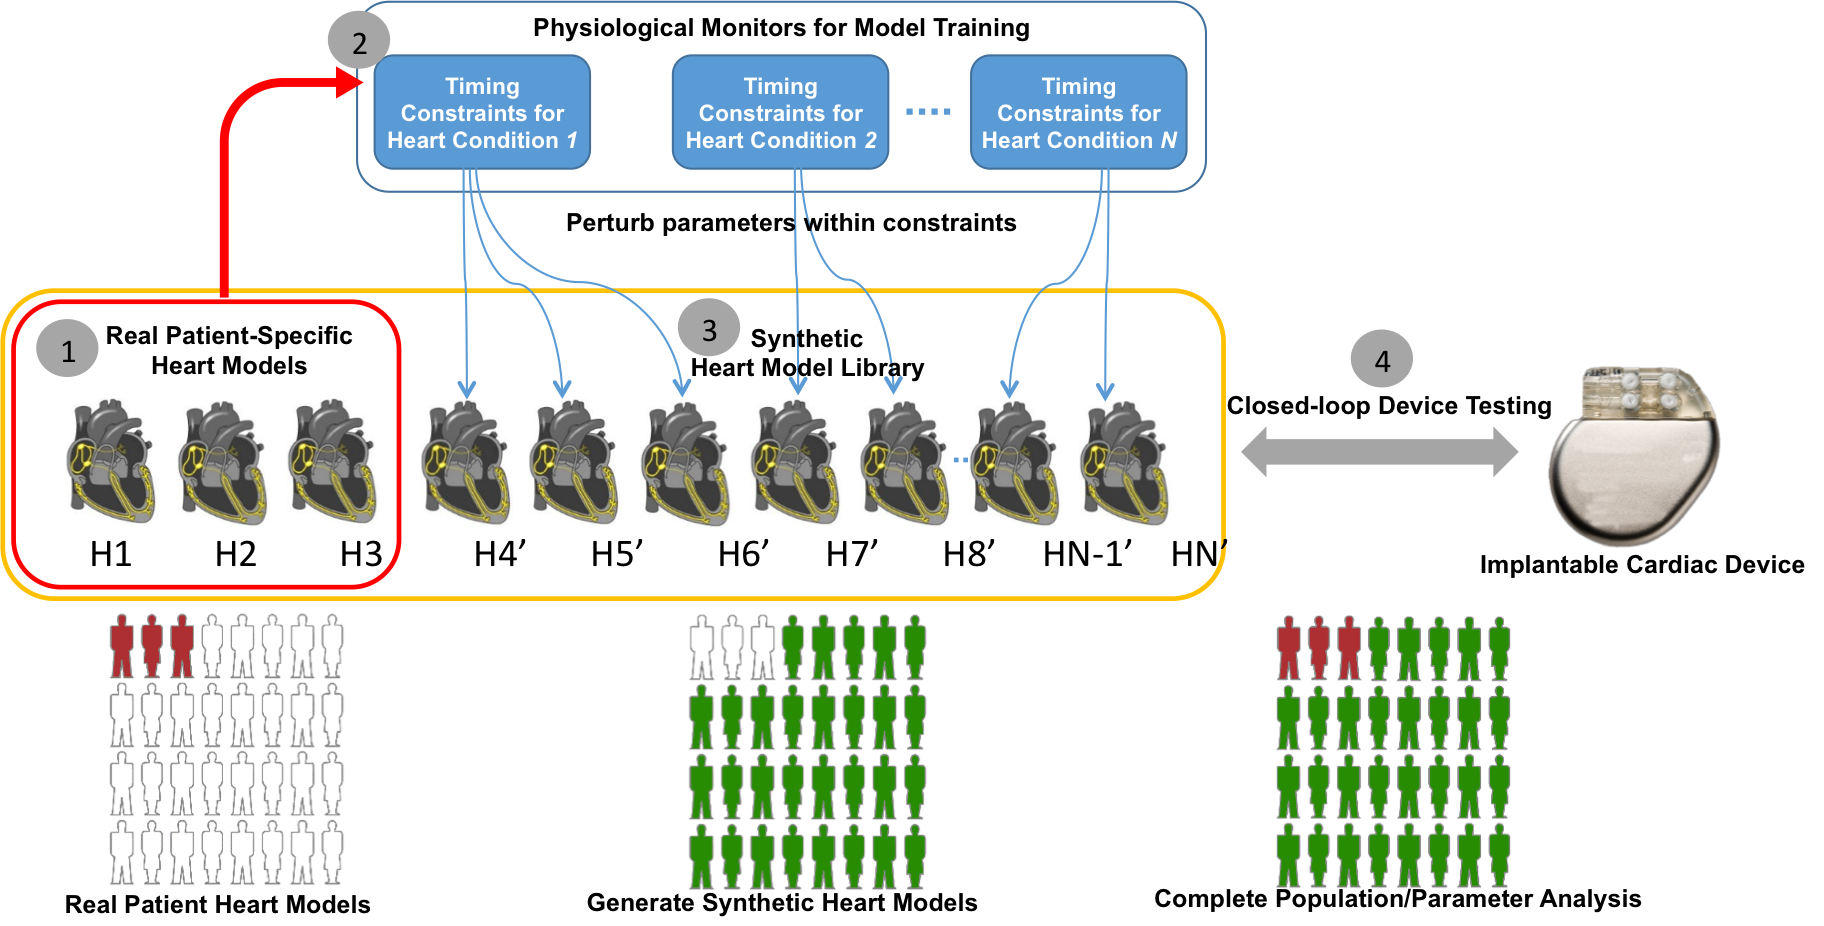
\includegraphics[width=\textwidth]{figs/fig5mbct.png}
	\caption{\small Model-based Clinical Trials}
	\label{fig:mbct}
\end{figure}
(The model cohort is the group of models enrolled in the trial).
Our current approach is to learn the constraints on parameters for the parametrized model using samples of real patients' data, as indicated by markers \circled{1} and \circled{2} in Fig. \ref{fig:mbct}. 
Ideally this sample of patients is a cohort from a previous trial.
These learned constraints are then used to generate more instances of the model (marker \circled{3}), and this constitutes our model cohort.
The device is then connected to these models (marker \circled{4}) and the outcomes of interest are evaluated, such as incidence of adverse events.

%Early efforts tying physiological modeling to clinical trials also include the  which is used to generate simulated patients.

\section{Conclusion}
\yhl{The safety and efficacy of closed-loop medical devices have to be evaluated within their physiological contexts.
In this article we demonstrated how physiological models can be used to provide safety evidence during the development of closed-loop medical devices, which can potentially safe time and cost for the device manufacturers.
Model-based clinical trials have the potential to reduce the scope, cost and probability of failure of clinical trials of medical devices with complex hardware and software. 
MBCT as a rapid certification toolchain to speed up medical device approvals is gaining increasing traction both within the regulatory environment and the medical device industry.
As an example, new diabetes control algorithms can be evaluated on the UVA/PADOVA diabetes model, and the result of which can be used to substitute animal trials \cite{pancreas_paul}. 
These applications can potentially usher a new era of exciting research challenges for the closed-loop verification, validation and testing medical devices at scale. 
}
\subsection{Heart Modeling}
 \label{sec:heart modeling}
The heart model has two components: a timing model and a morphology model.

\subsubsection{Timing Model}
\begin{figure}[t]
	\centering
	\vspace{-10pt}
	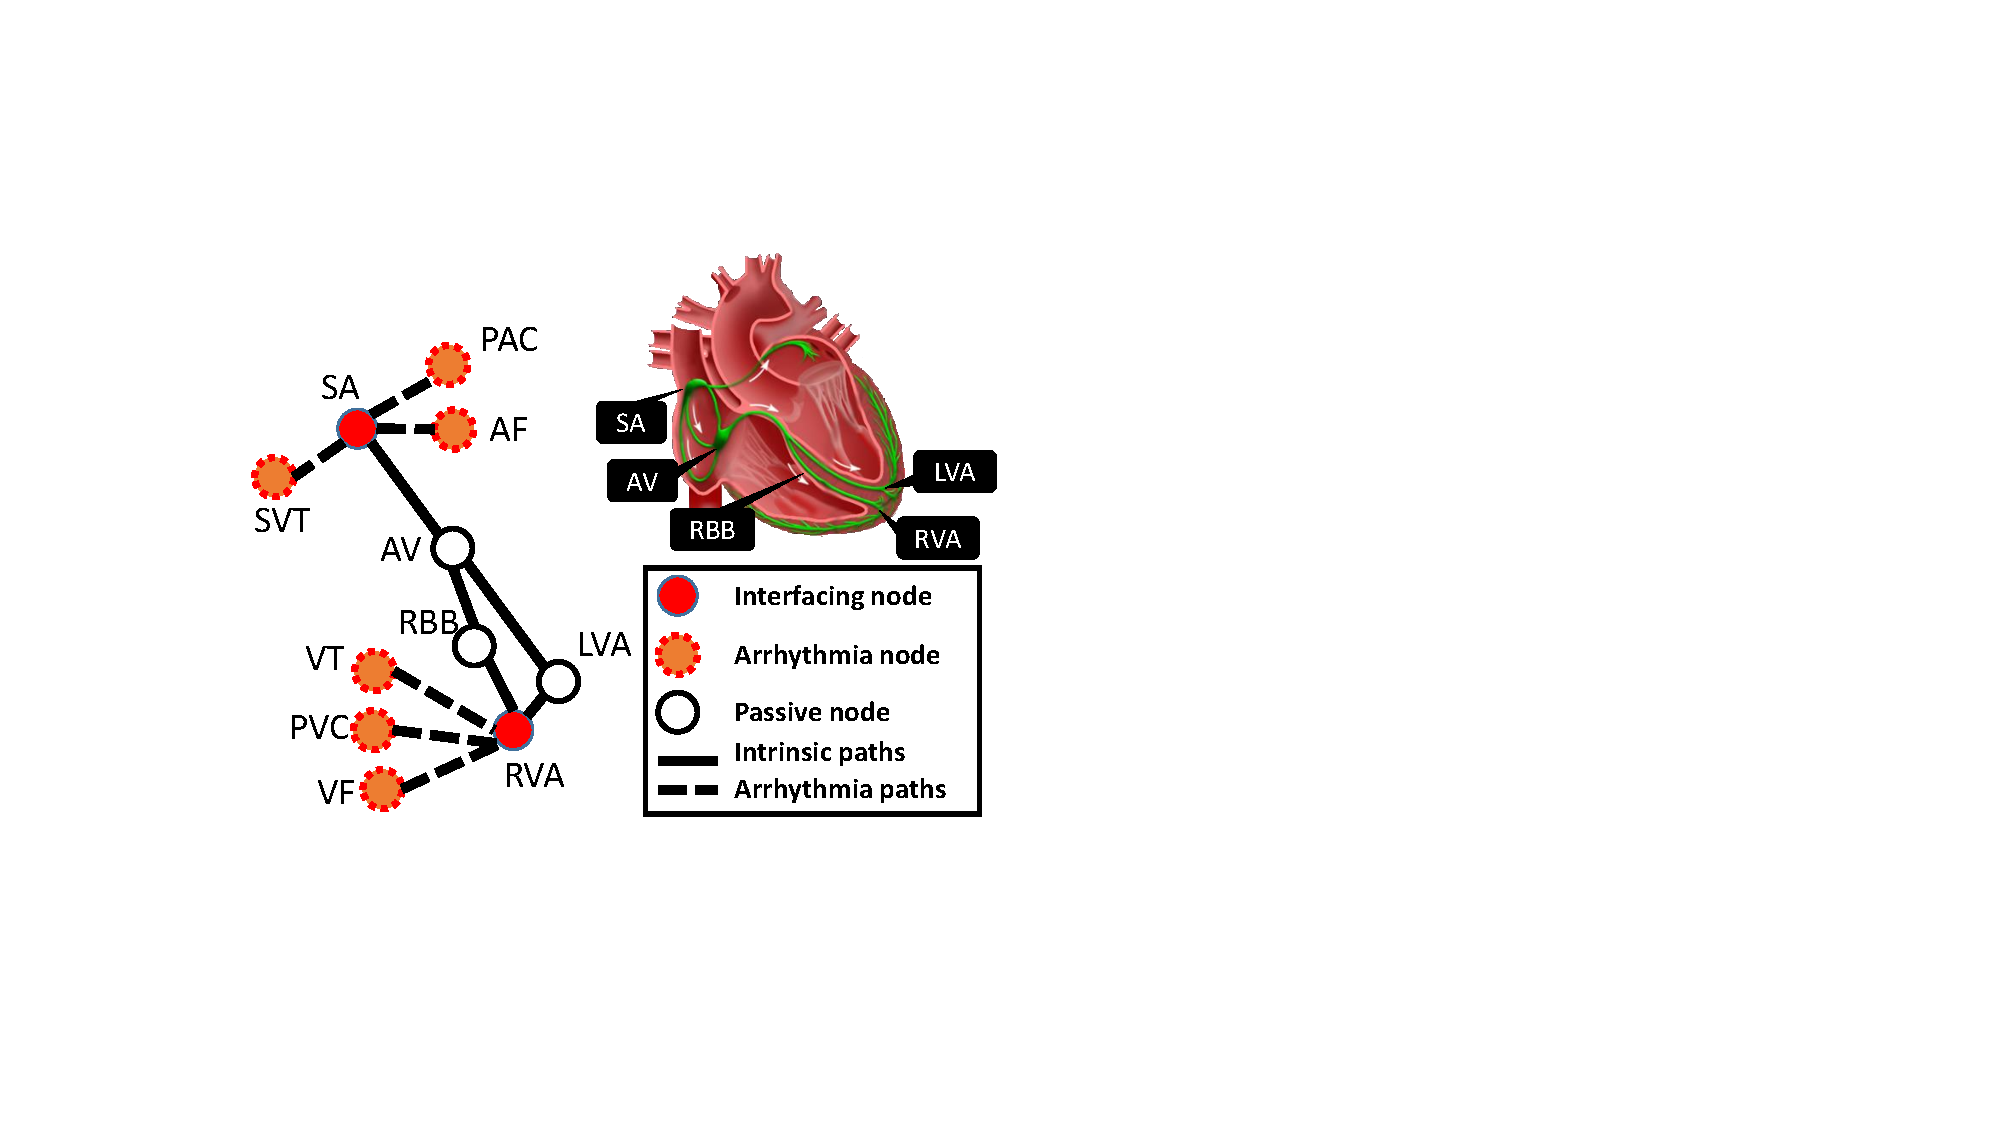
\includegraphics[width=0.3\textwidth]{figures/HM_top.pdf}
	\caption{\small Timing model of the heart}
	\vspace{-10pt}
	\label{fig:HM_top}
\end{figure}

Because the relative timing of atrial and ventricular events is an essential part of an arrhythmia's clinical definition, it is important that our model capture correctly the broad range of timings of various arrhythmias.
To this end, we developed an automaton model of the heart that simulates event sequences in atrium and ventricle shown in Fig. \ref{fig:HM_top}. 
Each filled node represents a potential source of spontaneous electrical activity, i.e., a potential source of an event.
For example, the SA node is the source of \ac{NSR}.
The \emph{dashed} filled nodes represent sources of \emph{abnormal} rhythms: e.g., the PAC node can produce Premature Atrial Complexes (a.k.a. ectopics), and the VF node can produce a ventricular fibrillation rhythm.

The hollow nodes (AV, RBBB, LVA) do not produce events. 
Rather, they are passive nodes representing key locations within the heart where electrical propagation may be blocked or delayed.
The paths connecting nodes represent bi-directional paths of propagation of electrical activity in the heart.
Thus an SA event propagates down to the RVA node via paths and the AV node, while a VF rhythm can propagate back to the atria via the LVA and AV nodes.

Each node and path has a set of timing parameters that control the rate, the delay between events, the conduction delay in a path, and how the rhythm changes from beat to beat, e.g., as a result of the refractory period.
By varying these parameters, we can simulate the timing of a wide variety of arrhythmias, and even vary the timing of a given arrhythmia beat-to-beat.
These timing parameters can be directly derived from clinical data \cite{josephson}, thus we know the ranges for these parameters.
In \cite{VHM_proc}, the timing model's capability to simulate various normal and abnormal heart conditions was validated quantitatively and by cardiac electrophysiologists. 
See Fig.~\ref{fig:mbct overview} \circled{2}.

\subsubsection{Morphology Model}
\emph{For a given patient}, it has been clinically observed that \ac{EGM} signals from the same source (i.e. the same location in the heart) generally have the same morphology. 
In our timing model, we have 5 different sources for SA node activation (the 5 dashed nodes connected to the SA node) and 5 different sources for RVA node activation (5 dashed nodes connected to the RVA node). 
Assume that we have a database of \acp{EGM}, where each \ac{EGM} has the distinctive morphology of that source, and is labeled with that source.
E.g., we have \acp{EGM} labeled `SA', others labeled `VF', etc.
(In next section, we explain how to build this database from real patients' data).
Given a sequence of atrial and ventricular events generated by the timing model, each event simply gets an \ac{EGM} that is labeled with that event's source (Fig. \ref{fig:egmGeneration}).
Concatenated, these give an entire arrhythmia episode.
To avoid repeating the exact same \ac{EGM}, which is unrealistic, we also introduce small variations on EGM templates.
The variations are obtained by a wavelet decomposition of the signatures followed by a random scaling of the 25\% smallest coefficients.
We guarantee that this does not change the labeling of the \ac{EGM} by running one of the morphology comparison discriminators used in the ICD.
See Fig.~\ref{fig:mbct overview} \circled{1}.

\begin{figure}[t]
	\centering
	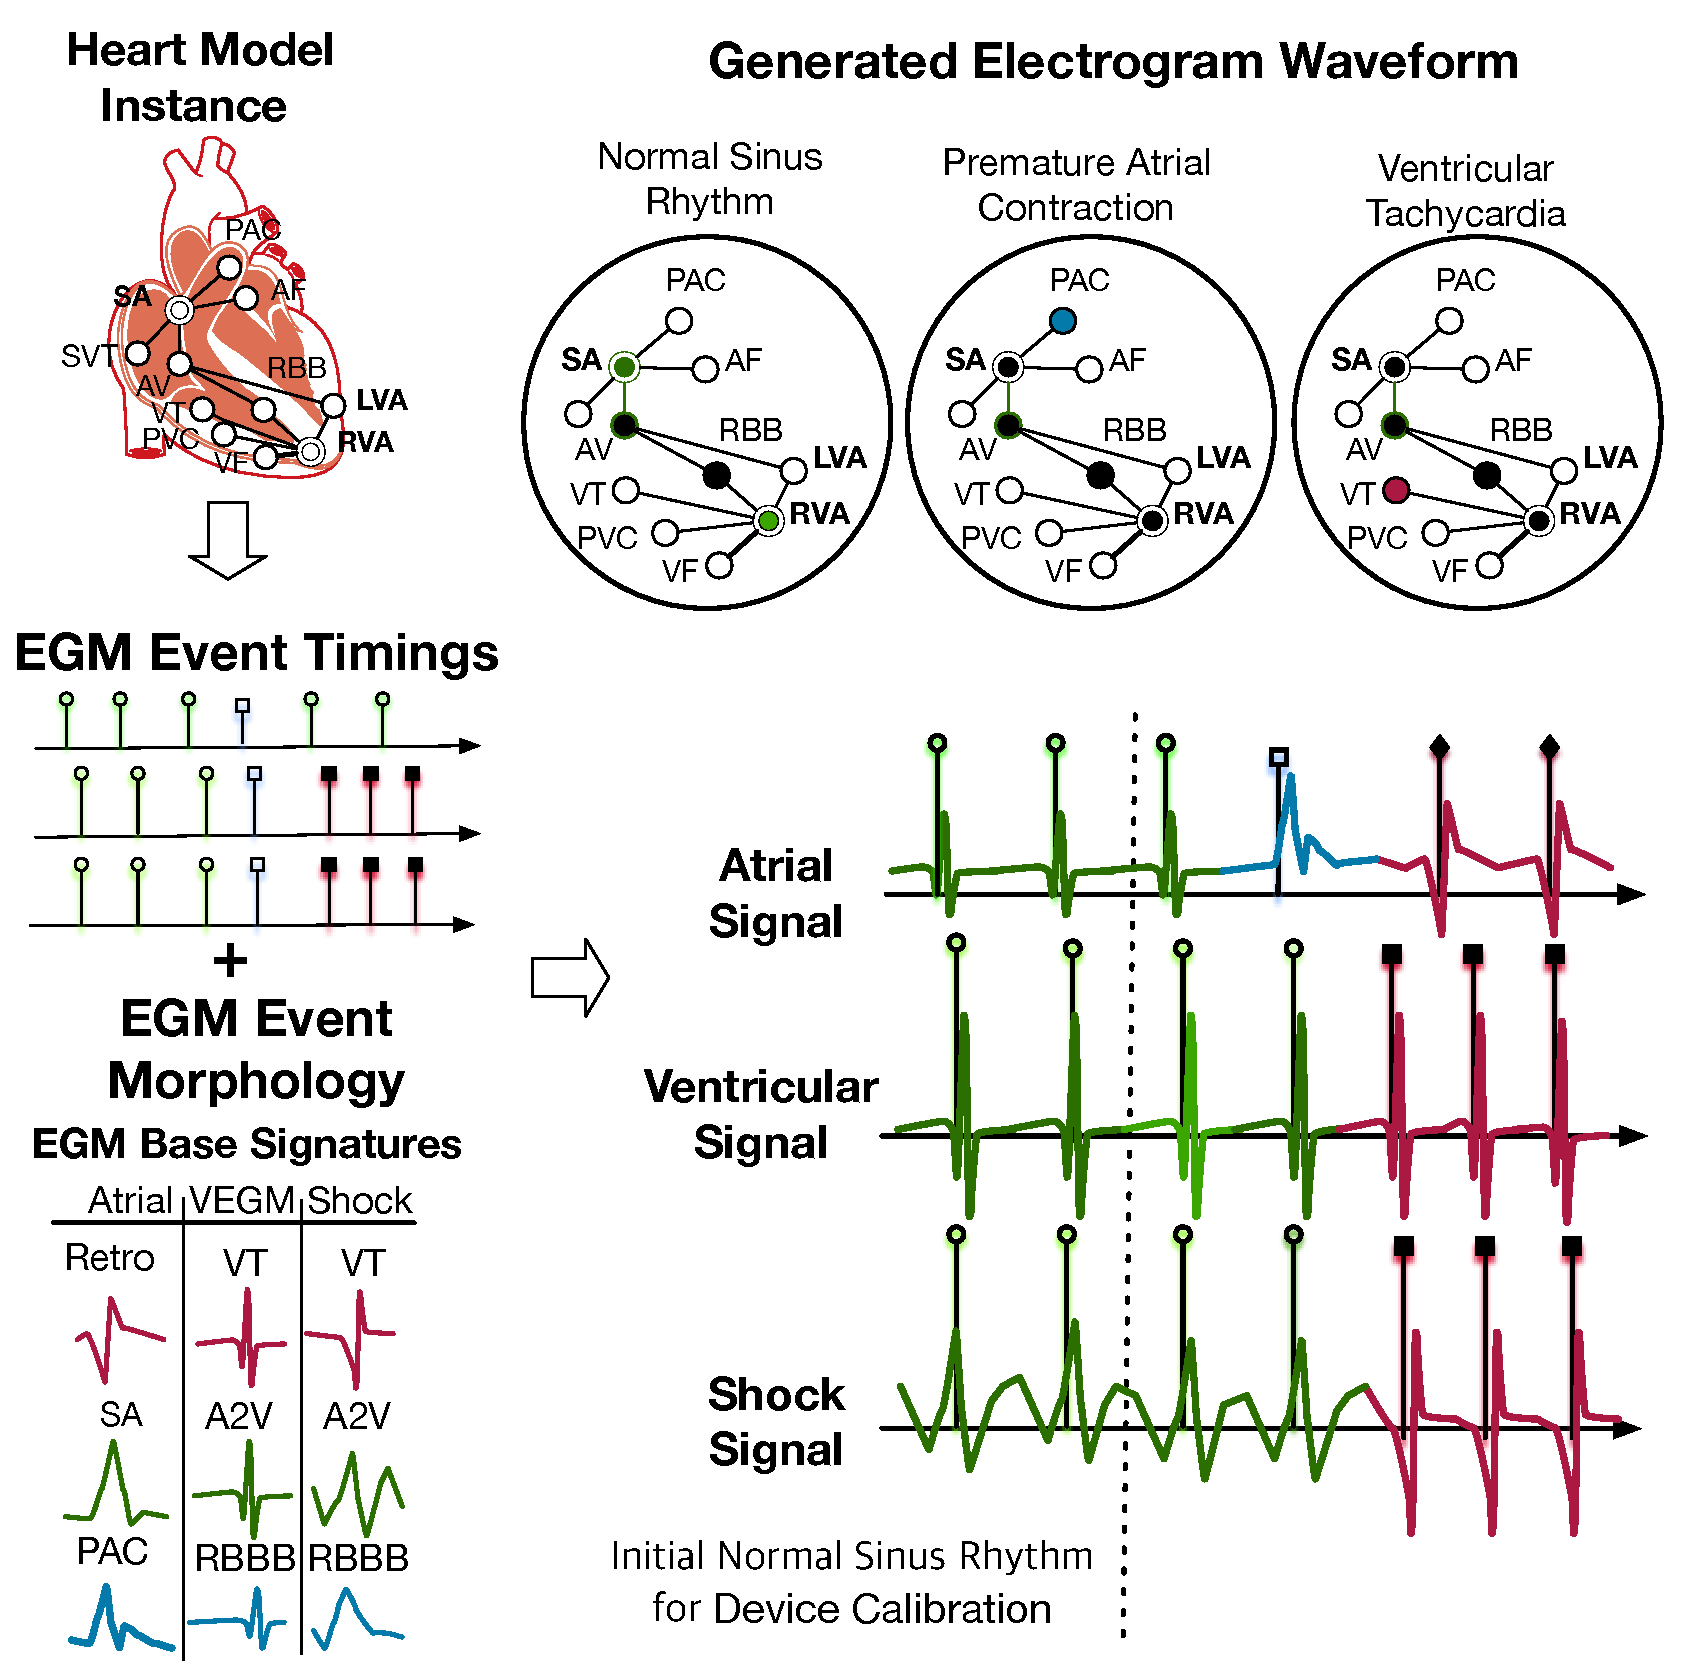
\includegraphics[scale=0.3]{figures/figEGMGeneration1column.pdf}
	\vspace{-15pt}
	\caption{\small \ac{EGM} waveform generation.
		From a given model instance and set of tachycardias, an EGM waveform is generated for the duration of an episode. The timing model determines event timings. When an event occurs, the EGM morphology for the event is output from the morphology model.  
		}
	\vspace{-15pt}
	\label{fig:egmGeneration}
\end{figure}

 \subsection{Patient Data Adjudication and EGM Template Extraction}
In order to obtain realistic morphologies for our simulations we utilize the Ann Arbor Electrogram Libraries (AAEL), a database of over 500 \ac{EGM} recordings made during clinical electrophysiology studies~\cite{AAEL}. 
The AAEL is used by all major \ac{ICD} manufacturers and is licensed by the US FDA. 
The AAEL provides descriptive annotations of records at a high level.
We performed additional detailed examination to precisely segment each record according to rhythm type.
123 records from 47 patients were manually examined and adjudicated into segments called \emph{episodes} containing one specific rhythm, e.g.\, \ac{NSR} or \ac{VF}. 
The adjudication was performed by a cardiologist.
Fig. \ref{fig:adjudication} (left) shows an example record (Record A185660) which has undergone this adjudication.
%It should be noted that only with a standard 12-lead \ac{ECG} in addition to ICD signals can all types of arrhythmia be accurately diagnosed.
From each episode, we developed an automated process which extracted \ac{EGM}s from a given episode. 
The \ac{EGM} are collected and organized by both patient record and by the type of rhythm which was annotated during the adjudication process.
These extracted rhythm \emph{signatures} provide the basis for the morphology information in the signal generated by our model.
Fig. \ref{fig:adjudication} (right) depicts an example of 10 signatures extracted from the record. 

\begin{figure*}[t]
	\centering
	\vspace{-10pt}
	\includegraphics[scale=0.35]{figures/figadjudication.pdf}
	\vspace{-10pt}
	\caption{\small  (Left) The \ac{EGM} record is segmented into episodes with distinct rhythms in each. (Right) From each episode, individual \acp{EGM} morphologies are extracted and stored.
	}
	\label{fig:adjudication}
\end{figure*}
%(Left) Adjudication of record A185660 
%(right) Examples of \ac{EGM} morphology signatures extracted from record: SA - Sinoatrial Node Event; Retrograde - Atrial event from Ventricular Retrograde; A2V - Sinus Atrial to Ventricular Conduction; A2V Shock - Shock signal of Sinus Atrial to Ventricular Conduction; PVC - Premature Ventricular Contraction Event; PVC Shock - Shock signal of Premature Ventricular Contraction Event; VT - \ac{VT} event; VT Shock - Shock signal of \ac{VT} event;  VF - \ac{VF} event; VF Shock - Shock signal of \ac{VF} event
%Our starting point is the AAEL database of \ac{EGM}s \cite{AAEL}.
%These are \ac{EGM} records collected from real patients during electrophysiologic testing.
%We worked with 123 records from 47 patients (a patient may have more than one recording session).
%We segmented each record into \emph{episodes}: an episode is a segment of a record with one main rhythm, e.g., Normal Sinus Rhythm or Ventricular Fibrillation.
%For a given rhythm, the database generally contains several episodes.
%Then from each episode of each rhythm, we extracted a number of electrograms, say, 10.
%The extracted \ac{EGM}s provide a \emph{signature} for what the \ac{EGM} looks like during that particular rhythm.
%Fig. \ref{fig:adjudication} illustrates the process of obtaining these signatures, as well as the extracted \ac{EGM}s and the rhythms of the episodes from which they were extracted.\begin{figure*}[t]
%		\centering
%		\includegraphics[scale=0.4]{figures/figadjudication.pdf}
%		\caption{\small Examples of \ac{EGM} morphology with different signatures.
%			 }
%		\label{fig:adjudication}
%\end{figure*}

\subsubsection{Cohort generation}
\label{sec:cohort generation}
See Fig.~\ref{fig:mbct overview}.
Let $p = (p_1,\ldots,p_n) \in \Re^n$ be the vector of parameters of the heart model.
Let $P_i \subset \Re$ be the range of parameter $p_i$.
We generate a \emph{synthetic cohort} of $N$ probabilistic model instances.
To produce one of these instances, for each scalar parameter $p_i$, we randomly select a sub-interval $I_i$ of its range: $I_i \subset P_i$.
The sub-interval $I_i$ is chosen so that it fits with the tachycardia that this model instance is meant to simulate.
E.g., for modeling \ac{VT}, the rest period of the \ac{VT} node might be assigned the sub-interval $I_i = [260, 280]ms$, reflecting the firing rate in the ventricles.
%Two different instances of the same tachycardia will, in general, have different sub-intervals within $P_i$.
When a model instance is simulated, each parameter $p_i$'s value changes beat to beat by sampling it uniformly within its sub-interval $I_i$.
Thus each generated model is probabilistic to reflect inherent rhythm variability.
\section{Implementing Device Algorithms} 
\label{sec:device models}
Due to the limited sensing capability of ICDs, device manufacturers have developed different algorithms to identify the electrical events and correctly diagnose the cardiac arrhythmia as being \ac{VT} or \ac{SVT}.
In this paper we implemented the detection algorithm Rhythm ID of Boston Scientific \cite{compass,Ellenbogen11_Pacingbook},% [???Compass, pacingdefibrillation,VTC paper, ICD book, Ellenbogen].
and PRLogic+Wavelet (PRL+W) of Medtronic \cite{Singer,Wavelet}.
%In available literature on the evaluations of device algorithms descriptions of the device algorithms are not detailed enough for full implementation.
%To obtain the detailed implementation we further reviewed clinical execution traces from literature like \cite{Singer} to infer detailed executions of the algorithms. 
We also set up a testing platform to validate our implementations against real ICDs using conformance testing.

\section{ICD Sensing}
\label{sec:sensing}
\begin{figure}[t]
	\centering
	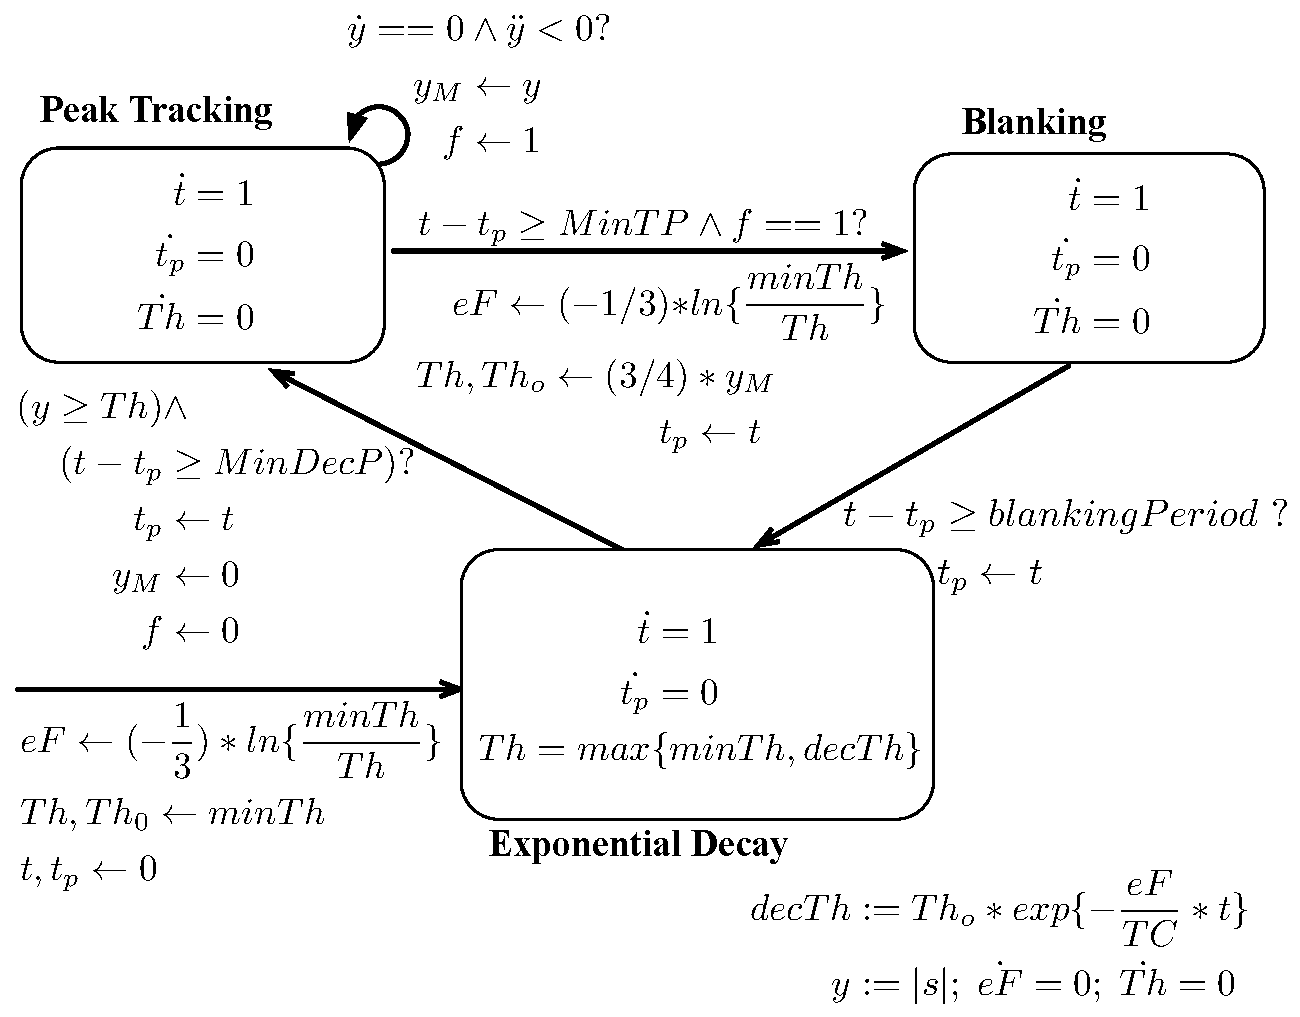
\includegraphics[scale=0.35]{figures/sensingModel}
	\vspace{-10pt}
	\caption{\small $\Sys_{Sense}$. States not shown in a mode have a 0 derivative, e.g., $\dot{eF}=0$ in all modes.}
	\vspace{-10pt}
	\label{fig:sensingModel}
\end{figure}
\begin{figure}[t]
	\centering
	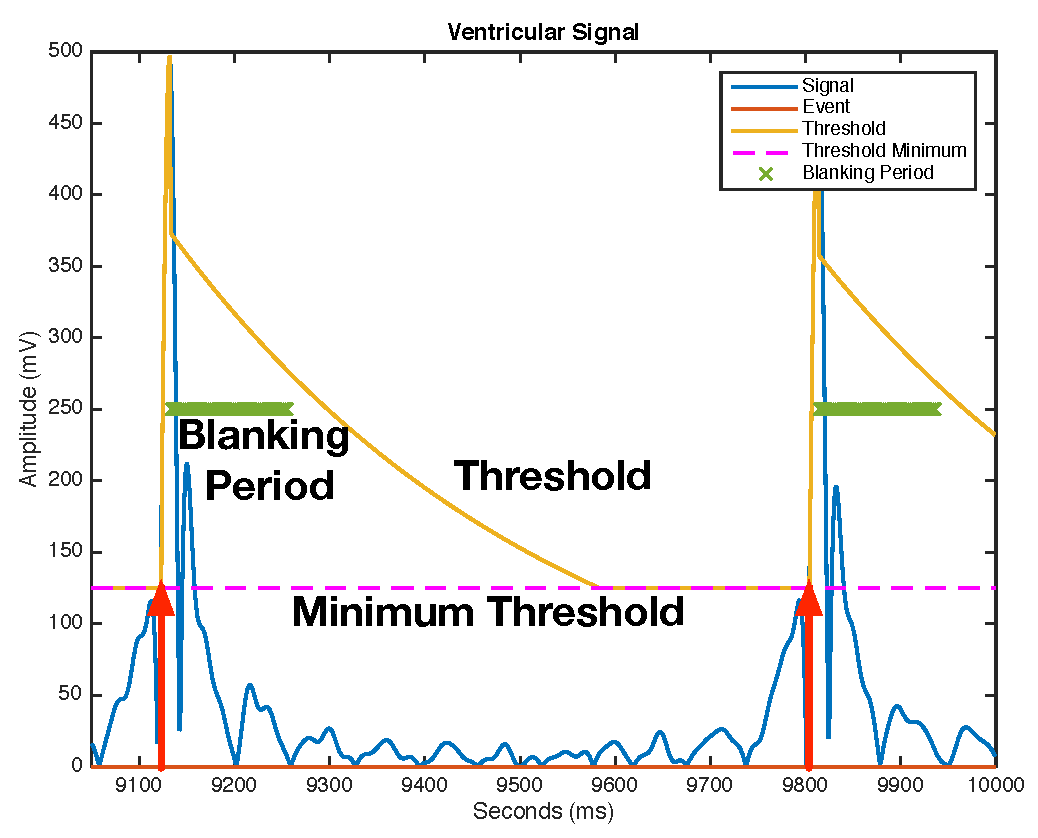
\includegraphics[scale=0.3]{figures/sensingExample}
	\vspace{-10pt}
	\caption{\small Example of dynamic threshold adjustment in ICD sensing algorithm. The shown signal is rectified.}
	\vspace{-10pt}
	\label{fig:sensingExample}
\end{figure}

\emph{Sensing} is the process by which cardiac signals $\egm$ measured through the leads of the \ac{ICD} are converted to cardiac timing events.
The \ac{ICD} sensing algorithm is a threshold-based algorithm which declares events when the signal exceeds a dynamically-adjusted threshold $Th$.
%The threshold is dynamically adjusted in order to operate robustly in complex environments where cardiac events can vary greatly in signal amplitude and frequency, such as during \ac{VF}.

Fig. \ref{fig:sensingModel} shows the model $\Sys_{Sense}$ of the sensing algorithm, and Fig. \ref{fig:sensingExample} illustrates its operation. 
%In Fig. \ref{fig:overview} (ICD Sensing - $\Sys_{Sense}$), states not shown in a mode have a 0 derivative, e.g., $\dot{eF}=0$ in all modes. $y(t) = |\egm(t)|$.
The sensing takes place on the rectified \ac{EGM} signal $y = |\egm|$.
After an event is declared at the current threshold value ($y(t)\geq Th(t)$ in Fig. \ref{fig:sensingModel}), the algorithm tracks the signal in order to measure the next peak's amplitude \yhl{(Peak Tracking)}.
%During transition, the state to indicate peak discovery is reset ($f=0$). 
For a duration $MinTP$ (min tracking period) the latest peak is saved in $y_M$.
A variable $f$ indicates that a peak was found.
After a peak is found ($f==1$) and after the end of the tracking period, the algorithm enters a fixed \emph{Blanking Period} \yhl{(Blanking)}, during which additional events are ignored.
\yhl{On the transition to Blanking}, $Th$ and $Th_0$ are set to 3/4 the current value of $y_{M}$ and the exponential factor of decay is updated ($eF=(-1/3)*ln{\frac{minTh}{TH}}$). 
At the end of the blanking period, the algorithm then transitions to the Exponential Decay mode in which $Th$ decays exponentially from $Th_0$ to a minimum level \yhl{(Exponential Decay)}:
$Th(t) = \max(minTh, Th_0\cdot exp(-(eF/TC)t)) $.
The algorithm stays in the Exponential Decay mode for at least a sampling period of $MinDecP$.
Correspondingly, there is a de facto Maximum Decay Period $MaxDecP$ after which the system transitions again to PeakTracking since the signal $y$ is bound to exceed the minimum threshold $minTh$.
Different manufacturers may use a step-wise decay instead of exponential, but the principle is the same.
%
Local peak detection is modeled via the $\dot{y} = 0 \wedge \ddot{y}<0$ transition.
While $y=|\egm|$ is non-differentiable at 0, the peak will occur away from 0, as shown in Fig. \ref{fig:sensingExample}.
The other states in Fig. \ref{fig:sensingModel} are $t, t_p$ (clocks).
$minTh$ and $TC$ are constant parameters.
\begin{thm}
	\label{thm:sensing}
	$\Sys_{Sense}$ is STORMED.	
\end{thm}
\begin{prf}
	\textbf{(S)} By definition, we only need to consider transitions between different modes to establish separability. 
	For all such transitions, there is a minimum dwell time in the mode before taking the transition, namely $MinTP$ in PeakTracking, $BlankingPeriod$ in Blanking, and  $MinDecP$ in mode ExponentialDecay.
	So the system is separable since there is a uniform minimum flow before jumping.
	\\
	\textbf{(T)} Flows are either constant, (piece-wise) linear, or piece-wise linear and exponential (in the case of $y$ and its derivatives) and therefore are TISG.
	\\
	\textbf{(O)} All the flows, resets and guard sets are definable in $\Lc_{\exp}$.
	(The absolute value and $\max$ functions can be broken down into boolean disjunctions of definable functions, and $t \mapsto \ln(t)$ is o-minimal by o-minimality of $\exp$).
	\\
	\textbf{(RM)} The state is $x = (t, t_p, y, y_M, f, Th, Th_0,eF) \in \Re^8$, and let 
	 $\phi = (\phi_t, \phi_{p}, \phi_y, \phi_m, \phi_f, \phi_{Th},\phi_0,\phi_{eF})$ be the corresponding $\phi$ vector.
	Recall that the \ac{EGM} voltage $\egm$, and so $y=|s|$, is upper-bounded by $V_M$.	
	\\ 
	\textbf{ExponentialDecay $\rightarrow$ PeakTracking}.
	Only $t_p,y_M$ and $f$ are modified, so monotonicity produces the constraint
	 $\phi_p(t-t_p) +\phi_m(0-y_M) + \phi_f(0-1) \stackrel{Want}{\geq} \varepsilon (|t-t_p|+|y_M|+1)$.
	We require the stronger constraint to hold:
	\[\phi_t MinDecP - \phi_m V_M -\phi_f \stackrel{Want}{\geq} \varepsilon(MaxDecP + V_M+1)\]
	\\
	\textbf{PeakTracking $\rightarrow$ PeakTracking}. Only $y_M$ and $f$ are reset. 
	Algebraic manipulation yields $-2V_M\phi_m + \phi_f \stackrel{Want}{\geq} \zeta$
	\\
	\textbf{PeakTracking $\rightarrow$ Blanking}.
	$t_p,eF,Th$ and $Th_0$ are reset, so we get
	\begin{eqnarray*}
	&&\;\phi_p(t-t_p) + \phi_{eF}(-(1/3)\ln(minTh/Th)-eF) 
	\\
	&&+\phi_{Th}(3y_M/4-Th) +\phi_0(3y_M/4-Th_0)
	\\
	&&\geq \varepsilon(|t-t_p|+ |-\frac{1}{3}\ln(\frac{minTh}{Th})-eF|
	\\
	&&+|\frac{3y_M}{4}-Th|+|\frac{3y_M}{4}-Th_0|)
	\end{eqnarray*}
	
	$Th$ is lower-bounded by $minTh$ at all times, and it is naturally upper-bounded by $V_M$ as the threshold should never exceed the largest possible attainable voltage. 
	By the same token, $0\leq eF \leq (1/3)\ln(V_M/minTh)$.
	Then we want the stronger inequality
	\begin{eqnarray*}
	\phi_p MinTP &+& \phi_{eF}(0-(1/3)\ln(V_M/minTh)
	\\
	&+&\phi_{Th}(-V_M) +\phi_0(-V_M)
	\\
	&\geq& \varepsilon(MaxTP+ |\frac{1}{3}\ln(\frac{V_M}{Th})|+|V_M|+|V_M|)
	\end{eqnarray*}
	\\
	\textbf{Blanking $\rightarrow$ ExponentialDecay}. Only $t_p$ is reset and therefore we want, $\phi_p(t-t_p) \geq \varepsilon(|t-t_p|)$, thus the transition yields $\phi_p \geq \varepsilon$.
	
	The above equations can be simultaneously satisfied.
	The simplest thing would be to set all $\phi$ terms that appear above to 0 except for $\phi_t,\phi_p$ which are calculated accordingly.
	
	The flows can be shown to be monotonic along the same $\phi$ and with the same $\varepsilon$.
	For example, in mode ExponentialDecay, only $t,y$ and $Th$ flow.
	Making use of the $V_M$ bound on $y$, we get the constraint
	$\phi_t \tau - 2V_M\phi_y +\phi_{Th}(Th(t+\tau)-Th(t))\geq \varepsilon(\tau+2V_M + |Th(t+\tau)-Th(t)| )$, 
	which yields $\phi_t \geq \varepsilon$, $\phi_y \leq -\varepsilon$ and $\phi_{Th} \geq \varepsilon$. 
	Similarly for the rest.	
\end{prf}

%\begin{thm}
%\label{thm:sensing}
%$\Sys_{Sense}$ is STORMED.	
%\end{thm}
%\begin{prf}
%\textbf{(S)} The guards are separable since each mode has only one guard.
%\\
%\textbf{(T)} The flows are constant, linear or equal to $\pm \egm(t)$ (in the case of $y$) and so are TISG.
%\\
%\textbf{(O)} All the flows, resets and guard sets are definable in $\Lc_{\exp}$.
%(The absolute value and $\max$ functions can be broken down into boolean disjunctions of definable functions).
%In particular, $t \mapsto \ln(t)$ is o-minimal by o-minimality of $\exp$.
%\\
%\textbf{(RM)} The only reset happens on the PeakTracking $\rightarrow$ Blanking transition. 
%The state is $x = (t,Th, eF,Th_0,t_p,y) \in \Re^5$.
%We seek a vector $\phi = (\phi_t, \phi_{Th}, \phi_{eF},\phi_0,\phi_y)$ and $\varepsilon >0$ s.t. 
%\begin{equation}
%\label{eq:sense rm}
%\phi \cdot \left(\begin{matrix}
%t-t \\ (3/4)Th-Th\\ -(1/3)\ln(minTh/Th) - eF\\ (3/4)Th-Th_0\\ t-t_p \\ y-y
%\end{matrix}
%\right) \defeq \phi \cdot \delta \stackrel{Want}{\geq} \varepsilon ||\delta||
%\end{equation} 
%$Th$ is lower-bounded by $minTh$ at all times, and it naturally has an upper bound, since it doesn't make sense to set it above the largest possible voltage. 
%Let that maximum be $maxTh$.
%Then we want the stronger inequality
%\begin{eqnarray*}
%&&\phi_{Th}(-Th/4) + \phi_{eF}(-(1/3)ln(minTh/Th)-eF) 
%\\
%&+& \phi_0(3Th/4-Th_0) + \phi_t (t-t_p) \geq ||\delta||
%\\
%&\geq& -\frac{\phi_{Th}}{4}maxTh + \phi_{eF}(-\frac{2}{3}\ln(minTh/Th)) 
%\\
%&& -\phi_0(2maxTh) + \phi_p(t-t_p)
%\\
%&\stackrel{Want}{\geq}& \varepsilon \left(|\frac{maxTh}{4}| + |\frac{2}{3}\ln(\frac{minTh}{Th})| + |2maxTh| +  \phi_p|t-t_p|\right)
%\end{eqnarray*}
%Since the $\ln$ term is negative and $t\geq t_p$,this yields the constraints:
%$\phi_0,\phi_{Th} < -\varepsilon \text{  and  } \phi_{eF},\phi_t > \varepsilon$.
%%\begin{equation}
%%\label{eq:constraint sense rm}
%%\phi_0,\phi_{Th} < -\varepsilon \text{  and  } \phi_{eF},\phi_t > \varepsilon
%%\end{equation}
%
%The flows are also monotonic along the same $\phi$ and with the same $\varepsilon$.
%For any $t,\tau>0$ and $x\in \stSet$, flow monotonicity is implied by the stronger inequality
%\begin{equation}
%\label{eq:sense fm}
%\phi \cdot \left(\begin{matrix}
%t+\tau-t \\ Th-Th\\ eF - eF\\ Th_0-Th_0\\ t_p-t_p \\ |\egm(t+\tau)|-|\egm(t)|
%\end{matrix}
%\right) \stackrel{Want}{\geq} \varepsilon (\tau + \underbrace{||\egm(t+\tau)|-|\egm(t)||}_{\delta \egm})
%\end{equation} 
%$\implies \phi_t \tau + \phi_y (|\egm(t+\tau)|-|\egm(t)|) \geq \varepsilon (\tau + \left| |\egm(t+\tau)|-|\egm(t)| \right| )$
%Therefore we can choose $\phi_t > \varepsilon$ as before and $\phi_y < -\varepsilon$.
%%We show this for Mode 1 only, the other modes are dealt with similarly.
%%\underline{Mode 1.} For any $t,\tau>0$ and $x\in \stSet$, flow monotonicity 
%%$\phi\cdot(\theta(t+\tau;x)-\theta(t;x)) \geq \varepsilon ||\theta(t+\tau;x)-\theta(t;x)||$ is implied by the stronger inequality
%%\begin{equation}
%%\label{eq:sense fm}
%%\phi \cdot \left(\begin{matrix}
%%t+\tau-t \\ Th-Th\\ eF - eF\\ Th_0-Th_0\\ t_p-t_p \\ -\egm(t+\tau)+\egm(t)
%%\end{matrix}
%%\right) \stackrel{Want}{\geq} \varepsilon (\tau + \underbrace{|\egm(t)-\egm(t+\tau)|}_{\delta \egm})
%%\end{equation} 
%%Observing that the \ac{EGM} signal $\egm$ has naturally defined minimum $\egm_{min}$ and maximum $\egm_{max}$, \eqref{eq:sense fm} is further implied by 
%%\begin{equation}
%%\phi_t\tau + \phi_y(\delta \egm) \geq \phi_t \tau - \phi_y(s_{min} -  s_{max}) \stackrel{Want}{\geq} \varepsilon (\tau +|s_{min} -  s_{max}|)
%%\end{equation}
%%which yields the constraints $\phi_t > \varepsilon, \phi_y < -\varepsilon$, which are consistent with \eqref{eq:constraint sense rm}.
%%The flow monotonicity constraints from the other modes are similarly consistent with \eqref{eq:constraint sense rm}. 
%\end{prf}

\subsection{VT Detection Algorithm}
\label{sec:svtvt}
%The limited sensing resolution and noise in the \ac{EGM} signals make it is impossible for the device to achieve 100\% accuracy for SVT/VT discrimination.
Device companies have developed different algorithmic components to distinguish \ac{SVT} from \ac{VT}, referred to as \emph{discriminators}. 
Each discriminator utilizes the history of timing and/or morphology of the EGM signals to determine whether the current rhythm is a \ac{VT} or \ac{SVT} (or neither).
%The decisions of each discriminators are then combined using a decision tree structure to decide whether to deliver or inhibit therapy.
No single discriminator is sufficient on its own to discriminate between \ac{SVT} and \ac{VT}, because these classes of arrhythmias can appear similar in a number of criteria.
Therefore discriminators are organized in a decision tree.%, as illustrated in Fig. \ref{fig:BS_det}.
We have implemented the detection algorithms Rhythm ID from Boston Scientific and PRL+W from Medtronic. 
This section gives an overview of both algorithms.

%We will need the following definition: an \emph{interval} is the amount of time between two consecutive electrical events. 
%Thus a ventricular interval is the duration between two ventricular events.
%Intervals are variable in length. 
%Consistently short intervals imply a fast rhythm.

\begin{figure*}[t]
	\centering
	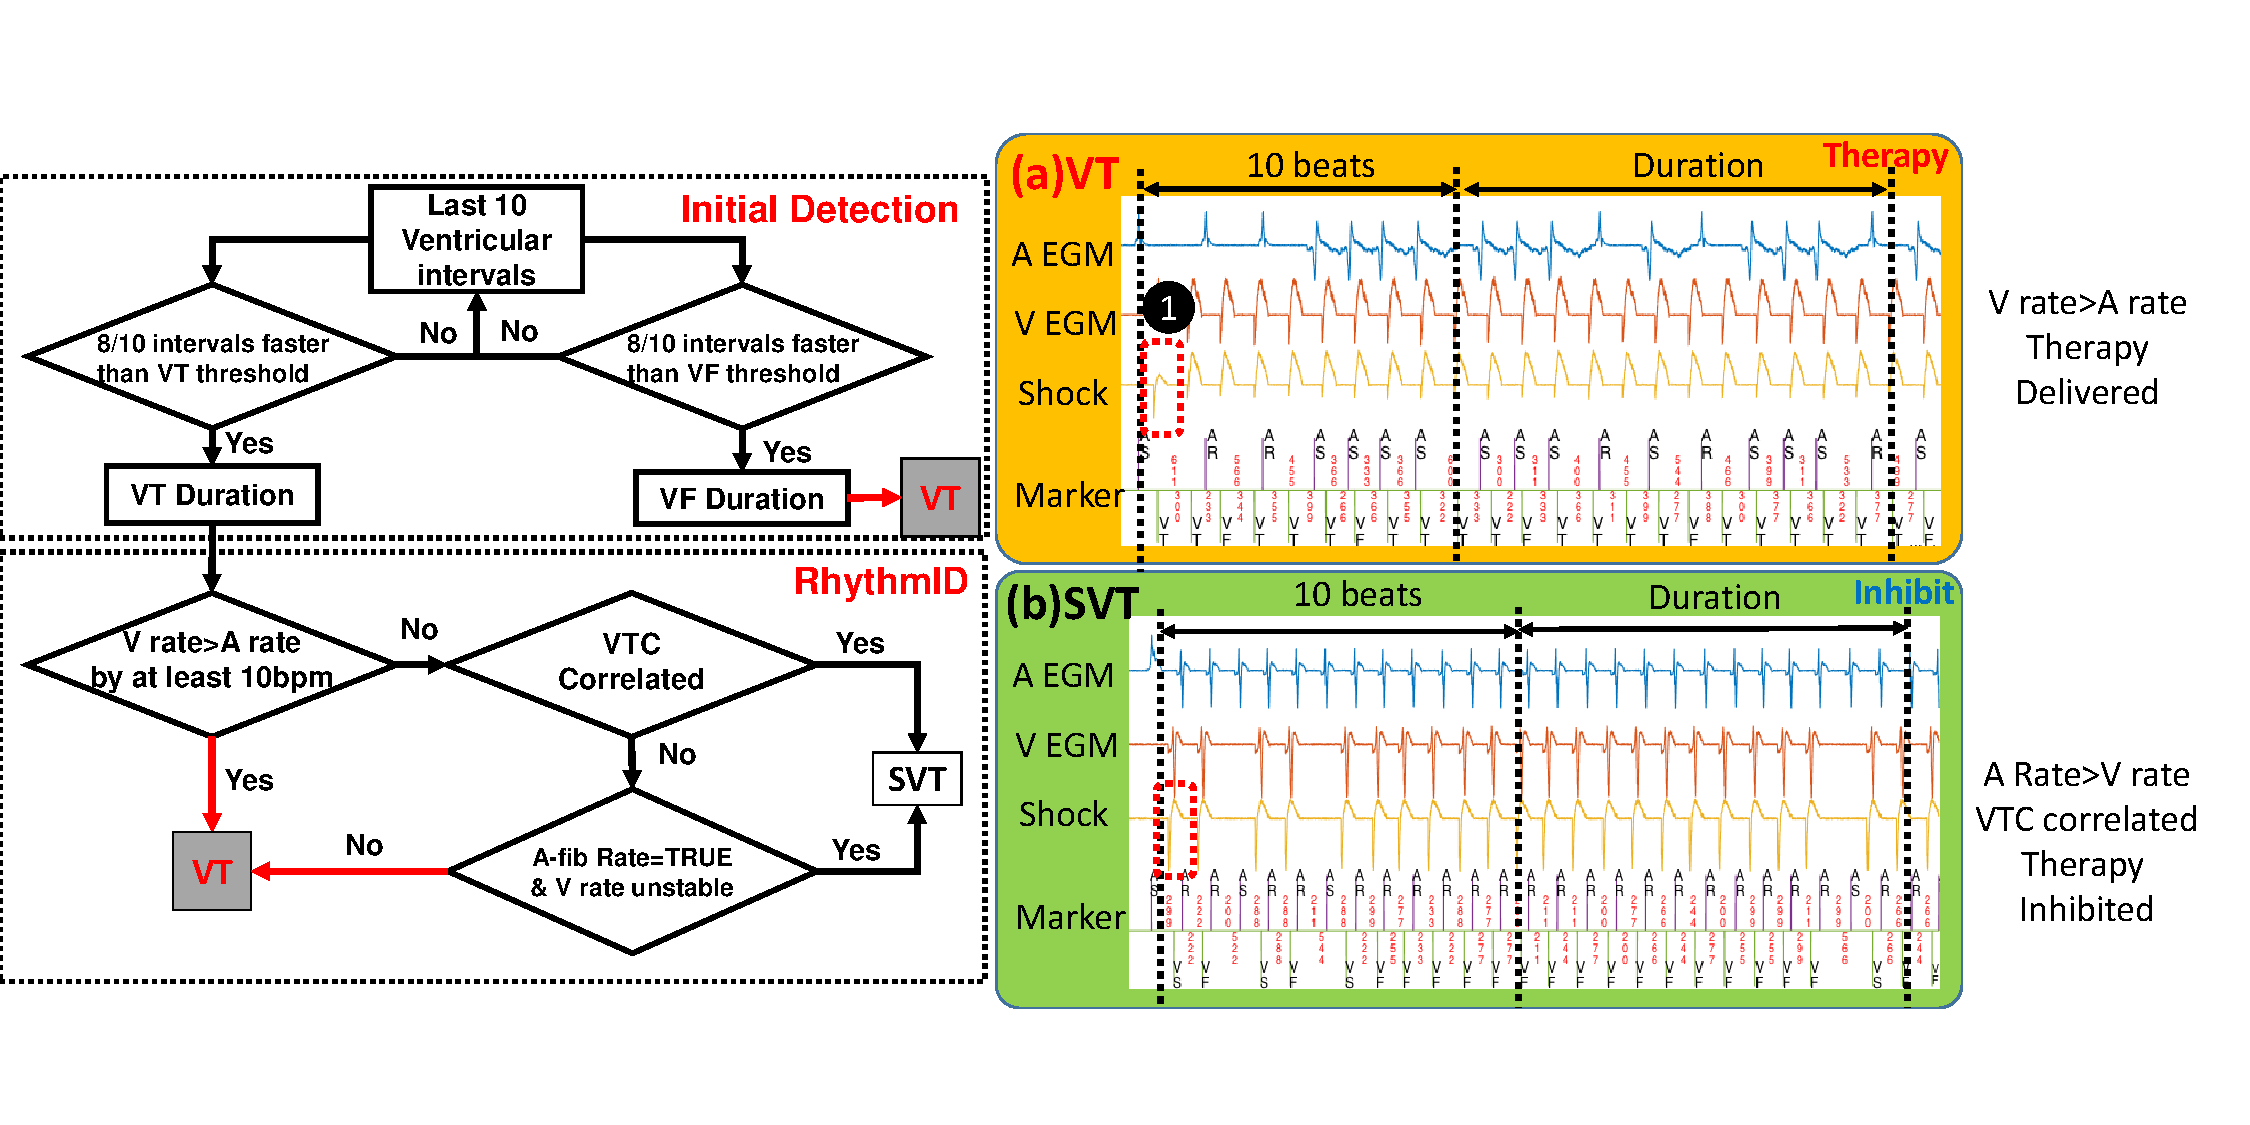
\includegraphics[scale=0.38]{figs/BS_det.pdf}
	\vspace{-10pt}
	\caption{\small SVT/VT detection algorithm by Boston Scientific \cite{compass}. The two cases on the right illustrate two different decisions by the algorithm. (a) illustrates a sustained VT case where at the end of the Duration, the ventricular rate is faster than the atrial rate. The algorithm correctly identified the rhythm as VT and delivered therapy. (b) illustrates a SVT case where at the end of the Duration, the ventricular rate is slower than the atrial rate. Then by comparing the EGM morphology in the Shock channel (Marker 1) with the stored NSR template (Marker 2) for the last 10 EGM events, the algorithm decided that the morphology is correlated, therefore therapy is inhibited.}
	\label{fig:BS_det}
\end{figure*}

\subsubsection{Rhythm ID}
Rhythm ID's decision tree is shown in Fig.~\ref{fig:BS_det}.
Rhythm ID detects an episode by continuously examining the last 10 ventricular intervals and comparing them with VT and VF thresholds. 
If 8/10 intervals are shorter than the VF threshold for a certain pre-set \emph{VF Duration} (e.g., 2.5 seconds) then the algorithm declares VF.
Otherwise, if 8/10 intervals are shorter than the VT threshold for a certain VT Duration, then further discriminators are used.
First, if the ventricular rate is greater than the atrial rate for the last 10 ventricular beats, Rhythm ID will determine the condition is VT.
Otherwise, the Vector Timing and Correlation (VTC) discriminator~\cite{VTC} compares EGM morphology of the last 10 ventricular events with an EGM \emph{template} saved during \ac{NSR}.
VTC is based on the assumption that the EGM morphology of the shock channel during VT is different from its morphology during SVT and NSR.
If the correlation between the current EGM's morphology and the stored NSR morphology is above a pre-set threshold, the current rhythm is more likely to be SVT than VT, and therapy is withheld.
Otherwise, if the atrial rate is equal to a pre-set fibrillation rate and the variance of the ventricular interval length exceeds a certain limit, the algorithm decides it's an \ac{SVT}. 
Otherwise, it decides this is a \ac{VT}.
%As shown in Fig. \ref{fig:BS_det}(b), at the end of the duration, the atrial rate is faster than the ventricular rate. 
%The morphology in the shock channel is similar to the NSR morphology (red dashed) so VTC is correlated and therapy is inhibited.
%As a comparison the morphology during VT is different from the NSR morphology (Marker 1 in Fig. \ref{fig:BS_det}).

\subsubsection{PR Logic+Wavelet}
PRL+W also utilizes rate-based and morphology-based discriminators similar (but not identical) to Rhythm ID.
The morphology discriminator used in PRL+W  is similar to VTC in Rhythm ID, but operates in the wavelet domain~\cite{Wavelet}.
PRL+W also continuously compares the pattern of atrial and ventricular activation to 19 pre-defined patterns~\cite{Singer}.
Each pattern is associated to a heart condition, like Sinus Tachycardia or \ac{VT}.
A match between the current activity and one of the pre-defined patterns is used as an indication that the current rhythm is explained by the associated condition.


\subsection{Validation}
\label{sec:validation}
%\begin{figure}[t]
%	\centering
%	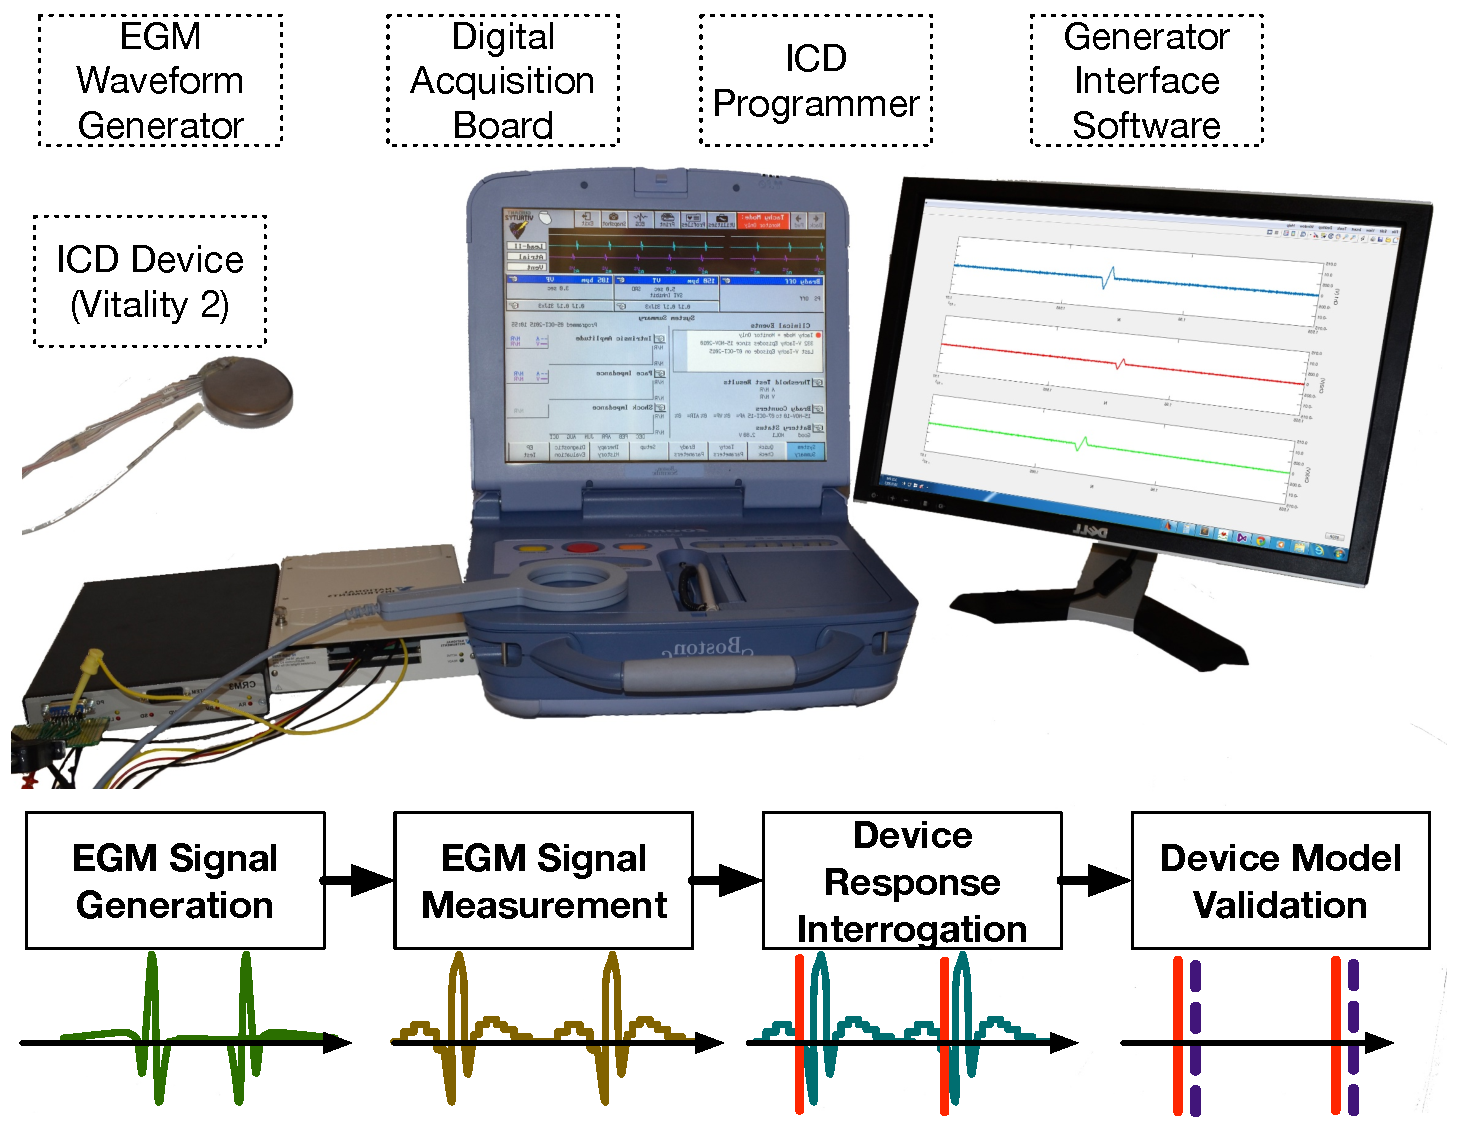
\includegraphics[scale=0.28]{figures/figValidationSetup.pdf}
%	\vspace{-10pt}
%	\caption{\small Model Validation. 14 different scenarios were generated from the EGM waveform generator for Boston Scientific and input into the Vitality 2 ICD. The input signal was acquired through the DAQ board and applied to the device model implementation. The ICD response was interrogated using the ICD programmer and compared to the output of the device model.}
%	\vspace{-10pt}
%	\label{fig:validationSetup}
%\end{figure}
\begin{figure}[t ]
	\centering
	\includegraphics[scale=0.28]{figures/figScreenshot.pdf}
	\caption{\small Example of validation output screenshots (Ventricular fibrillation) showing matching therapy decision for the ICD and our implementation.}
	\vspace{-10pt}
	\label{fig:validation}
\end{figure}

Conformance testing was used to validate the software implementations of the Vitality II device by Boston Scientific. 
The validation hardware setup is illustrated in Fig.~\ref{fig:validation}. 
14 different scenarios were specified and programmed into an EGM Waveform generator (CRM3 Simulator, Guidant, USA) such that it would output a signal to the connected Vitality II device.
The various scenarios traverse 7 out of 9 branches of the detection algorithm for Boston Scientific described in Sec. \ref{sec:svtvt} and shown in Fig. \ref{fig:BS_det}. 
The response of the \ac{ICD} interrogated using an ICD programmer (ZOOM Latitiude, Boston Scientific).
As the waveform was applied to the ICD, the waveform was simultaneously acquired using a National Instruments \ac{DAQ} board.
The recorded waveform was then applied to the device model and response was compared.
Fig. \ref{fig:validation} shows an example of one such scenario, specificallly \ac{VF}. 
In this case, the software model matched to the decision of the actual \ac{ICD} which also determined that therapy should be applied.

In all scenarios, the decision of model conformed to that of the \ac{ICD}. 
The remaining two branches were not reachable due to the limited output capability of the programmer.
The Medtronic software implementation can be validated using a similar process.

\section{Results}
\label{sec:results}
\subsection{The rate of inappropriate therapy}
\label{sec:rate inapp}
%\todo[inline]{justify episode-level rates and not patient-level}
The first objective of the MBCT is to estimate the rate of inappropriate detection $\bar{t}$ for each of the two algorithms for all arrhythmias combined, i.e., for the entire synthetic cohort.
The rate of inappropriate therapy is defined as
\[\bar{t} = \frac{\text{Number of inappropriately applied therapies}}{\text{Number of applied therapies}}\]
From this we can confirm or invalidate the assumption that Rhythm ID outperforms PRL+W.
We generated a synthetic cohort of 11,400 heart instances, equally distributed among the 19 arrhythmias.
The number of instances was obtained from a Monte Carlo calculation.% whose details follow the presentation of the results.

\textbf{Conclusion 1: PRL+W delivers less inappropriate therapy.}
The obtained rates of inappropriate detection were 6.65\% for Boston Scientific and 2.91\% for Medtronic (P < 0.0001), assuming an equal number of patients from each arrhythmia in the synthetic cohort.
The corresponding relative improvement \emph{of Medtronic over Boston Scientific} is 56\%.
In other words, the MBCT reveals that the PRL+W algorithm from Medtronic actually differentiates between VT and \ac{SVT} better than Rhythm ID from Boston Scientific.
Our findings are consistent with the observations of the RIGHT trial itself~\cite{GoldABBTB11_RIGHTresults}.

\textbf{Conclusion 2: result holds across population characteristics.}
The above rates were obtained under the assumption that each arrhythmia is equally represented in the cohort.
A significant feature of MBCT is that it allows us to study the endpoint of interest (here, rate of inappropriate detection) on a variety of populations, which have the various arrhythmias in different proportions.
This may not be feasible in a real clinical trial, which has to contend with the population present at the clinical centers where the trial is conducted.
We may then ask: does PRL+W maintain a lower rate of inappropriate detection across different populations?
To answer this question, we varied the distribution of the arrhythmias in the synthetic cohort, and re-computed the cohort-wide rates of inappropriate therapy.
Fig. \ref{fig:popvar8} shows the results for 10 random variations of the arrhythmia distribution.
It can be seen that indeed, PRL+W maintains a better rate of arrhythmia discrimination (and by inference, less inappropriate therapy) across the board.
%Thus the results are robust to the characteristics of the population under study.
%\mynote{SD}{Delete last sentence}

\begin{figure*}[t]
	\vspace{-10pt}
\centering
\vspace{-10pt}
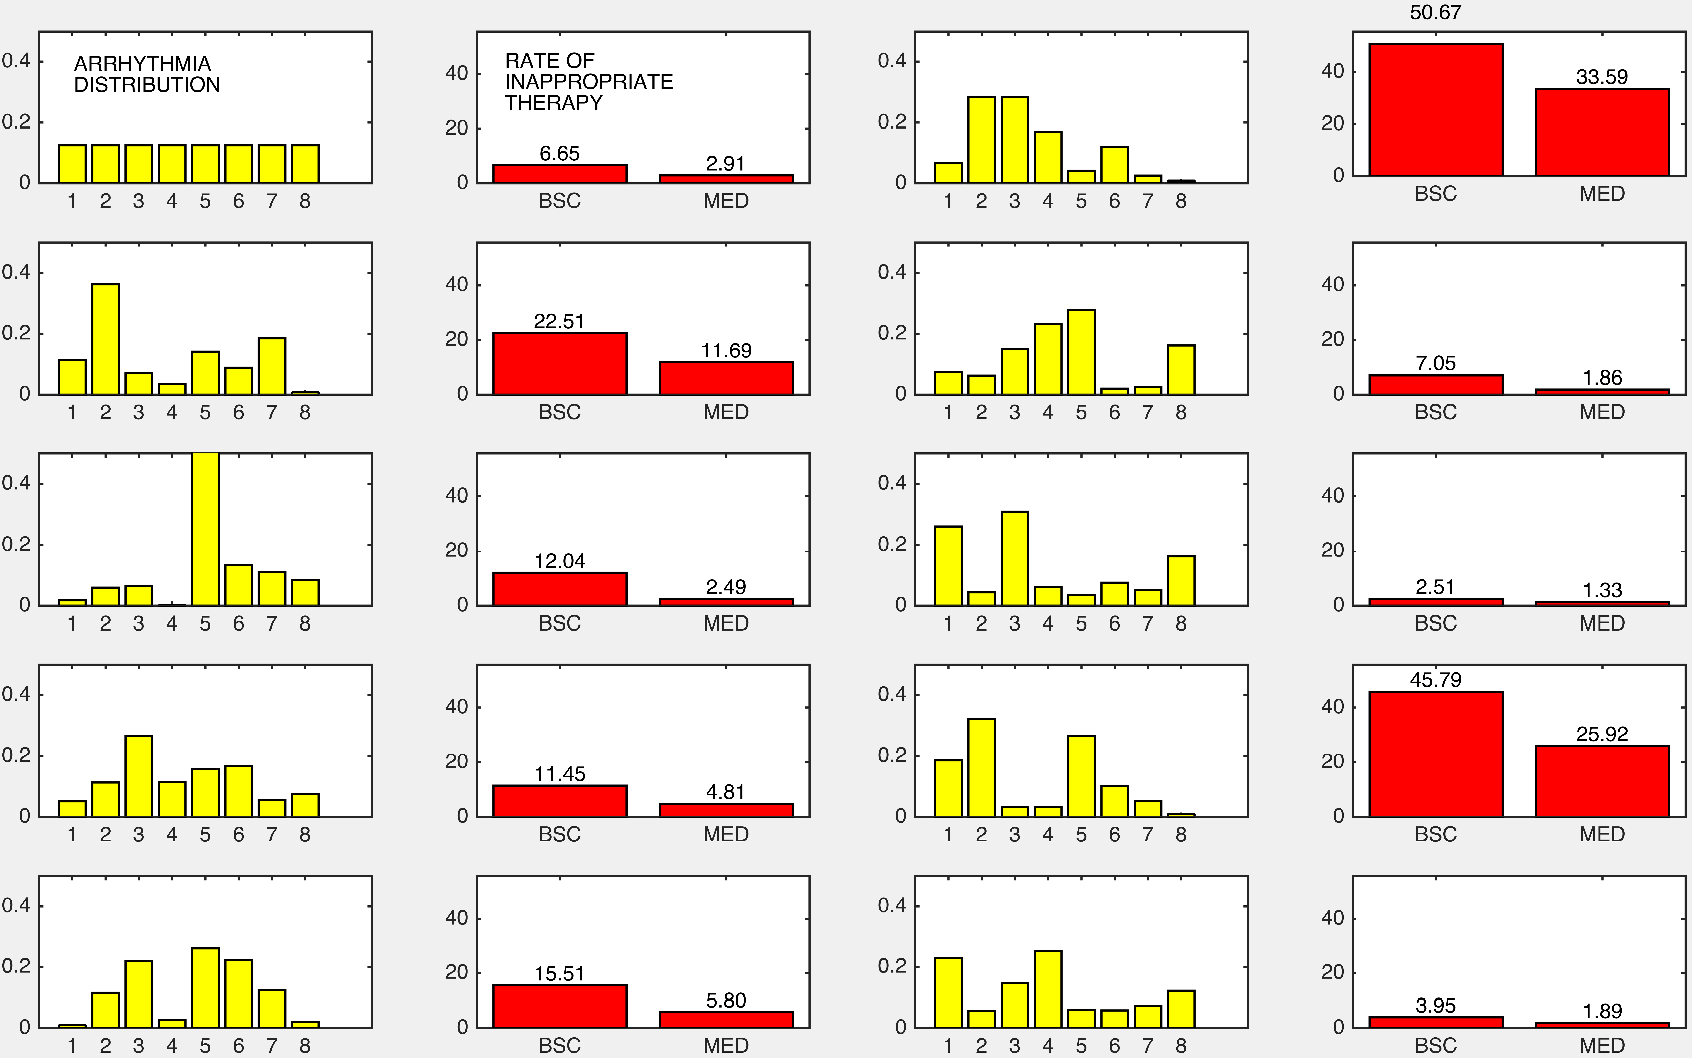
\includegraphics[scale=0.4]{figures/popvar9}
\caption{\small Rate of inappropriate detection ($2^{nd}$ and $4^{th}$ columns) for different arrhythmia distributions ($1^{st}$ and $3^d$ columns). The arrhythmias are (left to right on the x axis): Atrial fibrillation, Atrial flutter, Premature Ventricular Complexes, Nonsustained Ventricular Fibrillation, Supraventricular Tachycardia, Sinus Brady-Tachy, Ventricular Fibrillation, Ventricular Tachycardia \cite{josephson}. The top left distribution is uniform, and the bottom right distribution is that of the baseline characterization in RIGHT \cite{GoldABBTB11_RIGHTresults}.}
\label{fig:popvar8}
\end{figure*}

This illustrates very well the benefit that an \ac{MBCT} can bring to the planning of an \ac{RCT}: the fact that Rhythm ID could not be shown to be better than PRL+W %(let alone 25\% better as was hypothesized by the investigators) 
can cause the investigators to re-consider their assumptions and the feasibility of the trial.
In this case, the \ac{MBCT} casts doubt on the assumed \emph{direction} of the effect, i.e. whether intervention is better than control, or the other way around.
This early check can mean the difference between an expensive trial that fails at showing the desired effect, and a trial that is appropriately sized to demonstrate the desired effect size.

%While we will not know the true distribution of the arrhythmias in the \ac{RCT} until its completion, 
Thus, while an MBCT does not replace or mimic the RCT since we can not capture patient-level outcomes of the therapy, it can provide  but \emph{early insight} at a small fraction of the RCT cost and duration and without the ethical issues.	 

%\textbf{Sample size calculation for MBCT}.
%The rate is naturally computed as the mean of a random variable.
%Namely, it is the mean of the variable $t$ which equals 1 if the episode is a VT/VF for which therapy was applied, and 0 if it's a VT/VF for which therapy was withheld.
%To get reliable estimates for this rate, we use a standard Monte-Carlo calculation under the assumption that the estimate of the mean is normally distributed around the true mean. 
%This is justified by the central limit theorem and the fact that we can generate a very large number of hearts for each rhythm.
%By choosing a confidence interval width of 0.001 around the mean, we obtain a sample size of 9,604 hearts.
%In our experiments we used 11,400 to decrease the empirical variance of the estimate.
%The 95\% confidence interval around the mean estimate is given by $CI = \hat{t} \pm z_{95}\frac{S_t}{\sqrt{n}}$, 
%where $\hat{t}$ is the mean estimate, $z_c$ is the $c\%$ confidence level (so $z_{95}=1.96$), 
%$S_t$ is the empirical variance, 
%and $n$ is the number of Monte Carlo simulations, i.e., the number of heart instances we will generate and simulate for a given rhythm.
%The larger the number of simulations $n$, the tighter the confidence interval around the estimate.
%The rates we estimate fall in the range $[0,1]$ and are significant to the second decimal digit.
%Because we are considering all arrhythmias combined, we assume a conservative empirical variance $S_x$ to be 0.05, (validated experimentally) and set the desired confidence interval half-width to 0.001:
%\[\1.96\frac{0.05}{\sqrt{n}} = 0.001\]
%This yields $n = 9604$.
%In the experiments we use $n=11400$ to help guarantee the assumed empirical variance.
%The obtained empirical variance is invariably much smaller than 0.05.

%The obtained results for sensitivity and inappropriate therapy rate are shown 
%\begin{table}[b]
%	\smallcaption{Sensitivity and inappropriate therapy rate.}
%	\begin{tabular}{|p{1.9cm}|c|p{2.5cm}|}
%		\hline             & \textbf{Boston Sci.}(\%)   & \textbf{Medtronic} (\%)\\
%		\hline Sensitivity &  100                   &  100  \\ 
%		\hline Inappropriate therapy rate &  6.65                   &  2.91 \\ 
%		\hline 
%	\end{tabular}
%	\label{table:total nbs}
%\end{table} 

%We may also define a hypothesis test, which we illustrate for the rate of inappropriate therapy.
%The null hypothesis $H_{0,t}$ is that the rates for $\bar{t}$ are equal for Medtronic and Boston Scientific devices.
%\[H_{0,t}: \bar{t}_{MED} = \bar{t}_{BSC}  \]
%The alternative hypotheses are that the rates are not equal.
%In all that follows, `effect size' refers to the relative difference between the two rates.
%
%We assume an effect size of 27\%: this is based on the \emph{episode-level} inappropriate therapy rates reported in RIGHT (Table 2 of \cite{GoldABBTB11_RIGHTresults}).
%(Note that some of those reported results, however, were not statistically significant at the 5\% significance level).
%At the 5\% significance level and 90\% power, this yields a sample size of 11160.
%% with an assumed BSC rate of 0.08.
%We used 11400 instances in our MBCT.
%The results were inappropriate therapy rates $\bar{t}_{BSC}= 0.0291$ and $\bar{t}_{MED} = 0.0665$, with an effect size (relative to Medtronic's algorithm) of 56\% with $P << 10^{-3}$.
%Thus the null hypothesis of equality of inappropriate therapy rates can be rejected.

\subsection{Condition-level rates}
\label{sec:condition-level}
Having a heart model allows us to better estimate the \emph{sensitivity} and \emph{specificity} of the diagnostic algorithms' performance, something which is not possible in a clinical trial because the device only records a limited number of episodes.
These are defined as
\[ \text{Sensitivity} = \frac{\text{Number of correctly classified VTs}}{\text{Number of true VTs}}\]
\[ \text{Specificity} = \frac{\text{Number of correctly classified SVTs}}{\text{Number of true SVTs}}\]
In words, the sensitivity measures how well the device recognizes VTs.
Specificity measures how well the device discriminates between VT and SVT.
An ideal device would have 100\% sensitivity and specificity.
Unfortunately, these are typically competing goals: the more sensitive the device, the more likely it will mis-diagnose some SVTs as VTs, so its specificity will drop.
%During a clinical trial, the implanted ICD is typically set to record only treated episodes, so it is not possible to obtain all episodes and measure specificity.
%Moreover, if a VT episode is non-sustained, it won't receive therapy and won't be recorded, so it's not possible to measure sensitivity.
%Even if the device were set to record all episodes whether treated or not, memory limitations mean that it won't record everything.

We calculated sensitivity and specificity in our MBCT, and report them in Table \ref{table:vtsvt} on a per-arrhythmia basis.
The conditions are drawn from RIGHT's baseline characterization \cite{GoldABBTB11_RIGHTresults}.
Specificity is reported for SVTs and sensitivity is reported for VTs.
It can be seen from these results that in our synthetic cohort, Atrial flutter and other Supraventricular tachycardias are the main source of inappropriate detection for Rhythm ID compared to PRL+W.
In the case of Atrial flutter, Rhythm ID categorizes it inappropriately as \ac{VT} for 41.7\% of the cases.

Condition-level analysis pinpoints the specific pathways of the discrimination algorithm which must be addressed to reduce the device's rate of inappropriate therapy. It is difficult to get such insight through an RCT as the patient population is fixed and the conditions are determined retroactively. Such analysis can be further used to investigate condition distributions across different patient population types (e.g. abnormal heart rhythms in children vs geographic region-specific or race-specific condition distributions).   

\begin{table}[t]
	\vspace{-10pt}
	\smallcaption{Specificity and sensitivity.}
\begin{tabular}{|p{2.8cm}|p{1.5cm}|p{1.5cm}|c|}
	\hline Arrhythmia & Boston Sci. ICD & Medtronic ICDs  & P value \\ 
	\hline &	\multicolumn{2}{|c|}{\textbf{Specificity} (\%)}& \\
	\hline Atrial Fibrillation & 99.8 & 99.6 & 0.3167 \\ 
	\hline \cellcolor{blue!25} Atrial flutter & 58.3 & 79.33 & <0.0001 \\ 
	\hline Premature ventricular complexes & 100 & 100 & 1 \\ 
	\hline Nonsustained ventricular tachycardia & 100 & 99.8 & 0.3171 \\ 
	\hline \cellcolor{blue!25} Other Supraventricular tachycardia & 96.3 & 99.7 & <0.0001 \\ 
	\hline Brady-Tachy & 100 & 98.83 & 0.0079 \\ 
		\hline
	\hline &	\multicolumn{2}{|c|}{\textbf{Sensitivity} (\%)} & \textbf{P value}\\
	\hline Ventricular fibrillation & 100 & 100 & 1 \\ 
	\hline Ventricular tachycardia & 100 & 100 & 1 \\ 
	\hline 
\end{tabular} 
\vspace{-10pt}
\label{table:vtsvt}
\end{table}
 \subsection{Effect of Device Parameters on Discriminating Capability}
ICDs have a number of parameters which can be tuned to accommodate specific patient conditions by the physicians. 
%Currently there are very few clinical results on the effect of tuning parameters and their effect on sensitivity and specificity~\cite{maditrit}.
%One of the main causes of VT/SVT mis-classifications is inappropriate parameter settings~\cite{wrong_sensing}.
%In order for the physicians to set appropriate parameters, it is very important to understand how the change of one parameter can affect the discriminating capability of the device.
%With MBCT, one can use the same population across multiple devices with different parameter settings at virtually no cost. 
%The resulting trends can provide valuable insights to physicians.
In this section, we use MBCT to demonstrate the effects of changing two common parameters on SVT/VT discrimination specificity.
The first parameter is the \emph{\textbf{duration}} of arrhythmia before the ICD makes a therapy decision.
It is measured in seconds for Boston Scientific's devices, and in number of beats for Medtronic's devices. 
For Boston Scientific ICD the value can be set to 1 to 30 seconds.
%In this experiment we explore the values \{1,2,3,4,5,8,10\}.
%The equivalent parameter for Medtronic ICD is the number of consecutive fast ventricular intervals which can be set from 8 to 20 beats.
%In this experiment we explore the values \{8,10,12,16,18,24,30\} which roughly correspond to the parameters of Boston Scientific ICD.
%Intuitively, with a longer duration the device can examine a longer history of the arrhythmia episode, which can prevent inappropriate therapy, and thus increase SVT/VT discrimination specificity.
%Setting the duration too long can also cause missed therapies, thus affecting sensitivity. 
%These results are in agreement with the recently conducted ADVANCE-III RCT which showed that longer arrhythmia detection windows reduce shocks for Medtronic ICDs~\cite{advance3}.
%
The second parameter we vary is the \emph{\textbf{VF threshold}}.
For both devices, if the ventricular rate is faster than the VF threshold for a period of time the devices will deliver therapy without going into the SVT/VT detection algorithm. 
So a higher VF threshold means that more signals are passing through the discrimination algorithm.
%The value can be set to 150 to 200BPM.
%In this experiment we explore the value \{170,184,200\} for both devices.
%Intuitively the higher the threshold, the more episodes will be examined by the SVT/VT discrimination algorithm, which may increase specificity.
%However, VTs with rate less than the threshold may also be classified as SVT, causing missed therapies.\\

For each of the 21 parameter combinations described above, we ran a MBCT with 11,400 EGM episodes on both device models. 
Results are shown in Fig. \ref{fig:parameter}.
From the results we observe that for both devices the specificity increases monotonically with the length of the duration.
When the duration is longer than 5, sensitivities also dropped below 100\%, which is in line with the intuition.

\begin{figure}[t]
		\centering
		\vspace{-10pt}
		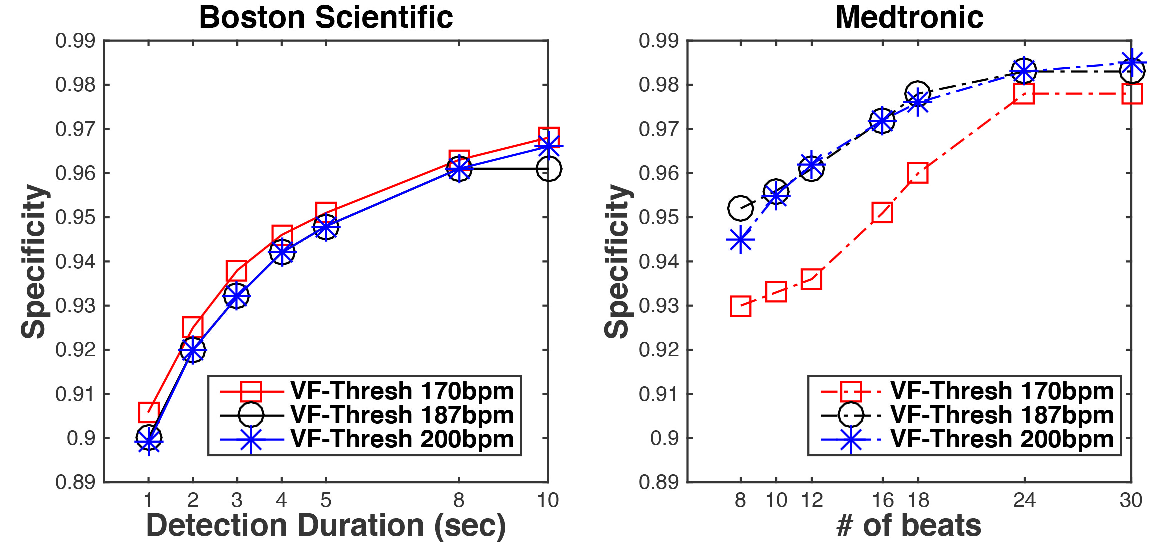
\includegraphics[width=0.45\textwidth]{figures/parameter.pdf}
		\caption{\small Effects of Duration and VF threshold parameters on Specificity}
		\vspace{-10pt}
		\label{fig:parameter}
\end{figure}

However, Boston Scientific algorithm and Medtronic algorithm displayed opposite trends for VF threshold.
%This agrees with the RIGHT finding that the rate of inappropriate therapy is highest for \acp{VT} with a rate $\leq 175$bpm \cite{GoldABBTB11_RIGHTresults}.
For Medtronic algorithm, the specificity increases when the VF threshold increases from 170BPM to 184BPM - i.e. a higher threshold admits more signals through the discrimination algorithm which performs better across all rates.
For Boston Scientific algorithm the specificity dropped when the VF threshold increases from 170BPM to 184BPM - i.e. the discrimination algorithm is less effective at higher rates. 
One possible interpretation of the result is that the Boston Scientific algorithm is more prone to inappropriate therapies for SVTs with ventricular rate between 170BPM to 184BPM, which is a very useful insight for the physicians to consider during parameter settings. 
%It should be noted that ICD settings are complex and studies across multiple parameter settings would need to be considered to provide conclusive guidance.








\subsection{Known lacunae in implementation}
\label{sec:discussion}
We did not account for post-shock detection (a phase of detection that follows the delivery of therapy), which was part of the RIGHT results.
We did not implement the Onset discriminator, which is part of the detection algorithms, so the results exclude its effects.
RIGHT included both dual-chamber and single-chamber devices, whereas we only implemented the algorithms for dual-chamber devices.
For the VTC and Wavelet algorithms, the literature did not specify which samples are taken from the electrogram. 
We chose to sample the electrogram uniformly in time, and validated that this gives correct results.
\section{Conclusion}
\label{sec:conclusion}

Clinical trials study the effect of an intervention \emph{in the patient}, and report patient-level results (e.g., ``The event of interest was observed in X\% of patients in Group 1''). 
Our results are at the condition level: they take the form ``the event of interest was observed in X\% of generated conditions".
To produce patient-level estimates requires an estimate of how conditions are distributed among patients. 
This low-level data is not publicly nor readily available.
A trial's investigators, however, should be able to obtain such data from previous trials.

It is important to stress that in general, one should not expect \emph{absolute numbers} from an MBCT to match those from a clinical trial, nor should this be the goal of the MBCT.
For example, in this work, it is unlikely that our MBCT will yield rates of inappropriate therapy that are equal to the rates obtained by RIGHT itself.
The reasons for this are many:
\begin{itemize}
	\item The RIGHT in vivo cohort, and our synthetic cohort, are not comparable:
	indeed, a myriad of factors affect the outcome of a clinical trial, e.g., whether some patients take up smoking. 
	These factors are not modeled.
	\item The adjudication of episodes in RIGHT (and other trials) is limited by the fact that only therapy episodes were recorded by the devices.
	The adjudication process is further limited by the lack of surface EKGs, which makes it hard to reliably distinguish certain atrial arrhythmias. 
	Neither of these is a limitation in MBCT since we have the ground truth: we know exactly what arrhythmia is being simulated by the model.  Furthermore, the AAEL signals have both device electrograms (EGMs) and the corresponding surface EKGs which allow for precise adjudication.  
	\item Experts may disagree on how to adjudicate the more complex episodes, so our classification of episodes from the AAEL database and the classification of the RIGHT investigators have an irreducible discrepancy.
	Again, this will affect the statistics that they and we compute.
\end{itemize}

That said, we can expect that a good heart model will reveal \emph{the trend} of the results, such as improvement of intervention over control or not, as shown in this paper. 
The MBCT conducted here clearly showed that the Medtronic algorithms outperforms the Boston Scientific's and resulted in a negative outcome of RIGHT across all population distributions and relevant heart conditions. In hindsight, the Boston Scientific-sponsored RIGHT would have needed reconsideration prior to running it to prevent a failed outcome.


%\keywords{ACM proceedings, \LaTeX, text tagging}
% The following two commands are all you need in the
% initial runs of your .tex file to
% produce the bibliography for the citations in your paper.
\bibliographystyle{unsrt}
\bibliography{biblio2}
% You must have a proper ".bib" file
%  and remember to run:
% latex bibtex latex latex
% to resolve all references
%
% ACM needs 'a single self-contained file'!

\end{document}

